\documentclass[twoside]{book}

% Packages required by doxygen
\usepackage{fixltx2e}
\usepackage{calc}
\usepackage{doxygen}
\usepackage[export]{adjustbox} % also loads graphicx
\usepackage{graphicx}
\usepackage[utf8]{inputenc}
\usepackage{makeidx}
\usepackage{multicol}
\usepackage{multirow}
\PassOptionsToPackage{warn}{textcomp}
\usepackage{textcomp}
\usepackage[nointegrals]{wasysym}
\usepackage[table]{xcolor}

% Font selection
\usepackage[T1]{fontenc}
\usepackage[scaled=.90]{helvet}
\usepackage{courier}
\usepackage{amssymb}
\usepackage{sectsty}
\renewcommand{\familydefault}{\sfdefault}
\allsectionsfont{%
  \fontseries{bc}\selectfont%
  \color{darkgray}%
}
\renewcommand{\DoxyLabelFont}{%
  \fontseries{bc}\selectfont%
  \color{darkgray}%
}
\newcommand{\+}{\discretionary{\mbox{\scriptsize$\hookleftarrow$}}{}{}}

% Page & text layout
\usepackage{geometry}
\geometry{%
  a4paper,%
  top=2.5cm,%
  bottom=2.5cm,%
  left=2.5cm,%
  right=2.5cm%
}
\tolerance=750
\hfuzz=15pt
\hbadness=750
\setlength{\emergencystretch}{15pt}
\setlength{\parindent}{0cm}
\setlength{\parskip}{3ex plus 2ex minus 2ex}
\makeatletter
\renewcommand{\paragraph}{%
  \@startsection{paragraph}{4}{0ex}{-1.0ex}{1.0ex}{%
    \normalfont\normalsize\bfseries\SS@parafont%
  }%
}
\renewcommand{\subparagraph}{%
  \@startsection{subparagraph}{5}{0ex}{-1.0ex}{1.0ex}{%
    \normalfont\normalsize\bfseries\SS@subparafont%
  }%
}
\makeatother

% Headers & footers
\usepackage{fancyhdr}
\pagestyle{fancyplain}
\fancyhead[LE]{\fancyplain{}{\bfseries\thepage}}
\fancyhead[CE]{\fancyplain{}{}}
\fancyhead[RE]{\fancyplain{}{\bfseries\leftmark}}
\fancyhead[LO]{\fancyplain{}{\bfseries\rightmark}}
\fancyhead[CO]{\fancyplain{}{}}
\fancyhead[RO]{\fancyplain{}{\bfseries\thepage}}
\fancyfoot[LE]{\fancyplain{}{}}
\fancyfoot[CE]{\fancyplain{}{}}
\fancyfoot[RE]{\fancyplain{}{\bfseries\scriptsize Generated by Doxygen }}
\fancyfoot[LO]{\fancyplain{}{\bfseries\scriptsize Generated by Doxygen }}
\fancyfoot[CO]{\fancyplain{}{}}
\fancyfoot[RO]{\fancyplain{}{}}
\renewcommand{\footrulewidth}{0.4pt}
\renewcommand{\chaptermark}[1]{%
  \markboth{#1}{}%
}
\renewcommand{\sectionmark}[1]{%
  \markright{\thesection\ #1}%
}

% Indices & bibliography
\usepackage{natbib}
\usepackage[titles]{tocloft}
\setcounter{tocdepth}{3}
\setcounter{secnumdepth}{5}
\makeindex

% Hyperlinks (required, but should be loaded last)
\usepackage{ifpdf}
\ifpdf
  \usepackage[pdftex,pagebackref=true]{hyperref}
\else
  \usepackage[ps2pdf,pagebackref=true]{hyperref}
\fi
\hypersetup{%
  colorlinks=true,%
  linkcolor=blue,%
  citecolor=blue,%
  unicode%
}

% Custom commands
\newcommand{\clearemptydoublepage}{%
  \newpage{\pagestyle{empty}\cleardoublepage}%
}

\usepackage{caption}
\captionsetup{labelsep=space,justification=centering,font={bf},singlelinecheck=off,skip=4pt,position=top}

%===== C O N T E N T S =====

\begin{document}

% Titlepage & ToC
\hypersetup{pageanchor=false,
             bookmarksnumbered=true,
             pdfencoding=unicode
            }
\pagenumbering{roman}
\begin{titlepage}
\vspace*{7cm}
\begin{center}%
{\Large vcvj \\[1ex]\large 0.\+1.\+0 }\\
\vspace*{1cm}
{\large Generated by Doxygen 1.8.11}\\
\end{center}
\end{titlepage}
\clearemptydoublepage
\tableofcontents
\clearemptydoublepage
\pagenumbering{arabic}
\hypersetup{pageanchor=true}

%--- Begin generated contents ---
\chapter{Namespace Index}
\section{Namespace List}
Here is a list of all documented namespaces with brief descriptions\+:\begin{DoxyCompactList}
\item\contentsline{section}{\hyperlink{namespacevcvj}{vcvj} }{\pageref{namespacevcvj}}{}
\item\contentsline{section}{\hyperlink{namespacevcvj_1_1_exceptions}{vcvj.\+Exceptions} }{\pageref{namespacevcvj_1_1_exceptions}}{}
\item\contentsline{section}{\hyperlink{namespacevcvj_1_1_models}{vcvj.\+Models} }{\pageref{namespacevcvj_1_1_models}}{}
\item\contentsline{section}{\hyperlink{namespacevcvj_1_1_models_1_1_enums}{vcvj.\+Models.\+Enums} }{\pageref{namespacevcvj_1_1_models_1_1_enums}}{}
\item\contentsline{section}{\hyperlink{namespacevcvj_1_1_models_1_1_grammatical___components}{vcvj.\+Models.\+Grammatical\+\_\+\+Components} }{\pageref{namespacevcvj_1_1_models_1_1_grammatical___components}}{}
\item\contentsline{section}{\hyperlink{namespacevcvj_1_1_models_1_1_grammatical___subcomponents}{vcvj.\+Models.\+Grammatical\+\_\+\+Subcomponents} }{\pageref{namespacevcvj_1_1_models_1_1_grammatical___subcomponents}}{}
\item\contentsline{section}{\hyperlink{namespacevcvj_1_1_parsers}{vcvj.\+Parsers} }{\pageref{namespacevcvj_1_1_parsers}}{}
\end{DoxyCompactList}

\chapter{Hierarchical Index}
\section{Class Hierarchy}
This inheritance list is sorted roughly, but not completely, alphabetically\+:\begin{DoxyCompactList}
\item \contentsline{section}{vcvj.\+Models.\+Grammatical\+\_\+\+Subcomponents.\+Color\+Table}{\pageref{classvcvj_1_1_models_1_1_grammatical___subcomponents_1_1_color_table}}{}
\begin{DoxyCompactList}
\item \contentsline{section}{vcvj.\+Models.\+Grammatical\+\_\+\+Subcomponents.\+Global\+Color\+Table}{\pageref{classvcvj_1_1_models_1_1_grammatical___subcomponents_1_1_global_color_table}}{}
\item \contentsline{section}{vcvj.\+Models.\+Grammatical\+\_\+\+Subcomponents.\+Local\+Color\+Table}{\pageref{classvcvj_1_1_models_1_1_grammatical___subcomponents_1_1_local_color_table}}{}
\end{DoxyCompactList}
\item \contentsline{section}{vcvj.\+Models.\+Grammatical\+\_\+\+Components.\+Data\+Block}{\pageref{classvcvj_1_1_models_1_1_grammatical___components_1_1_data_block}}{}
\begin{DoxyCompactList}
\item \contentsline{section}{vcvj.\+Models.\+Grammatical\+\_\+\+Components.\+Graphic\+Block}{\pageref{classvcvj_1_1_models_1_1_grammatical___components_1_1_graphic_block}}{}
\item \contentsline{section}{vcvj.\+Models.\+Grammatical\+\_\+\+Components.\+Special\+Purpose\+Block}{\pageref{classvcvj_1_1_models_1_1_grammatical___components_1_1_special_purpose_block}}{}
\begin{DoxyCompactList}
\item \contentsline{section}{vcvj.\+Models.\+Grammatical\+\_\+\+Subcomponents.\+Application\+Extension}{\pageref{classvcvj_1_1_models_1_1_grammatical___subcomponents_1_1_application_extension}}{}
\item \contentsline{section}{vcvj.\+Models.\+Grammatical\+\_\+\+Subcomponents.\+Comment\+Extension}{\pageref{classvcvj_1_1_models_1_1_grammatical___subcomponents_1_1_comment_extension}}{}
\end{DoxyCompactList}
\end{DoxyCompactList}
\item \contentsline{section}{vcvj.\+Models.\+Grammatical\+\_\+\+Components.\+Data\+Stream}{\pageref{classvcvj_1_1_models_1_1_grammatical___components_1_1_data_stream}}{}
\item Exception\begin{DoxyCompactList}
\item \contentsline{section}{vcvj.\+Exceptions.\+Application\+Extension\+Parser\+Exception}{\pageref{classvcvj_1_1_exceptions_1_1_application_extension_parser_exception}}{}
\item \contentsline{section}{vcvj.\+Exceptions.\+Unidentified\+Block\+Exception}{\pageref{classvcvj_1_1_exceptions_1_1_unidentified_block_exception}}{}
\end{DoxyCompactList}
\item \contentsline{section}{vcvj.\+Models.\+Grammatical\+\_\+\+Subcomponents.\+Graphic\+Control\+Extension}{\pageref{classvcvj_1_1_models_1_1_grammatical___subcomponents_1_1_graphic_control_extension}}{}
\item \contentsline{section}{vcvj.\+Models.\+Grammatical\+\_\+\+Components.\+Graphic\+Rendering\+Block}{\pageref{classvcvj_1_1_models_1_1_grammatical___components_1_1_graphic_rendering_block}}{}
\begin{DoxyCompactList}
\item \contentsline{section}{vcvj.\+Models.\+Grammatical\+\_\+\+Components.\+Table\+Based\+Image}{\pageref{classvcvj_1_1_models_1_1_grammatical___components_1_1_table_based_image}}{}
\item \contentsline{section}{vcvj.\+Models.\+Grammatical\+\_\+\+Subcomponents.\+Plain\+Text\+Extension}{\pageref{classvcvj_1_1_models_1_1_grammatical___subcomponents_1_1_plain_text_extension}}{}
\end{DoxyCompactList}
\item \contentsline{section}{vcvj.\+Models.\+Grammatical\+\_\+\+Subcomponents.\+Header}{\pageref{classvcvj_1_1_models_1_1_grammatical___subcomponents_1_1_header}}{}
\item \contentsline{section}{vcvj.\+Models.\+Grammatical\+\_\+\+Subcomponents.\+Image\+Data}{\pageref{classvcvj_1_1_models_1_1_grammatical___subcomponents_1_1_image_data}}{}
\item \contentsline{section}{vcvj.\+Models.\+Grammatical\+\_\+\+Subcomponents.\+Image\+Descriptor}{\pageref{classvcvj_1_1_models_1_1_grammatical___subcomponents_1_1_image_descriptor}}{}
\item \contentsline{section}{vcvj.\+Models.\+Grammatical\+\_\+\+Components.\+Logical\+Screen}{\pageref{classvcvj_1_1_models_1_1_grammatical___components_1_1_logical_screen}}{}
\item \contentsline{section}{vcvj.\+Models.\+Grammatical\+\_\+\+Subcomponents.\+Logical\+Screen\+Descriptor}{\pageref{classvcvj_1_1_models_1_1_grammatical___subcomponents_1_1_logical_screen_descriptor}}{}
\item \contentsline{section}{vcvj.\+Models.\+Grammatical\+\_\+\+Subcomponents.\+Trailer}{\pageref{classvcvj_1_1_models_1_1_grammatical___subcomponents_1_1_trailer}}{}
\item \contentsline{section}{vcvj.\+Vcvj\+Image}{\pageref{classvcvj_1_1_vcvj_image}}{}
\end{DoxyCompactList}

\chapter{Class Index}
\section{Class List}
Here are the classes, structs, unions and interfaces with brief descriptions\+:\begin{DoxyCompactList}
\item\contentsline{section}{\hyperlink{classvcvj_1_1_models_1_1_grammatical___subcomponents_1_1_application_extension}{vcvj.\+Models.\+Grammatical\+\_\+\+Subcomponents.\+Application\+Extension} \\*An extension which contains application-\/specific instructions, including the number of times an animated G\+IF image should loop. }{\pageref{classvcvj_1_1_models_1_1_grammatical___subcomponents_1_1_application_extension}}{}
\item\contentsline{section}{\hyperlink{classvcvj_1_1_exceptions_1_1_application_extension_parser_exception}{vcvj.\+Exceptions.\+Application\+Extension\+Parser\+Exception} }{\pageref{classvcvj_1_1_exceptions_1_1_application_extension_parser_exception}}{}
\item\contentsline{section}{\hyperlink{classvcvj_1_1_models_1_1_grammatical___subcomponents_1_1_color_table}{vcvj.\+Models.\+Grammatical\+\_\+\+Subcomponents.\+Color\+Table} \\*A block containing information about colors used. Can be global or local (frame-\/specific). }{\pageref{classvcvj_1_1_models_1_1_grammatical___subcomponents_1_1_color_table}}{}
\item\contentsline{section}{\hyperlink{classvcvj_1_1_models_1_1_grammatical___subcomponents_1_1_comment_extension}{vcvj.\+Models.\+Grammatical\+\_\+\+Subcomponents.\+Comment\+Extension} \\*An extension containing a comment. }{\pageref{classvcvj_1_1_models_1_1_grammatical___subcomponents_1_1_comment_extension}}{}
\item\contentsline{section}{\hyperlink{classvcvj_1_1_models_1_1_grammatical___components_1_1_data_block}{vcvj.\+Models.\+Grammatical\+\_\+\+Components.\+Data\+Block} \\*A generic data block representing either a graphic block or a special purpose block. }{\pageref{classvcvj_1_1_models_1_1_grammatical___components_1_1_data_block}}{}
\item\contentsline{section}{\hyperlink{classvcvj_1_1_models_1_1_grammatical___components_1_1_data_stream}{vcvj.\+Models.\+Grammatical\+\_\+\+Components.\+Data\+Stream} }{\pageref{classvcvj_1_1_models_1_1_grammatical___components_1_1_data_stream}}{}
\item\contentsline{section}{\hyperlink{classvcvj_1_1_models_1_1_grammatical___subcomponents_1_1_global_color_table}{vcvj.\+Models.\+Grammatical\+\_\+\+Subcomponents.\+Global\+Color\+Table} \\*A block containing global information about colors used. }{\pageref{classvcvj_1_1_models_1_1_grammatical___subcomponents_1_1_global_color_table}}{}
\item\contentsline{section}{\hyperlink{classvcvj_1_1_models_1_1_grammatical___components_1_1_graphic_block}{vcvj.\+Models.\+Grammatical\+\_\+\+Components.\+Graphic\+Block} \\*A block containing a graphic-\/rendering block and an optional graphic control extension. }{\pageref{classvcvj_1_1_models_1_1_grammatical___components_1_1_graphic_block}}{}
\item\contentsline{section}{\hyperlink{classvcvj_1_1_models_1_1_grammatical___subcomponents_1_1_graphic_control_extension}{vcvj.\+Models.\+Grammatical\+\_\+\+Subcomponents.\+Graphic\+Control\+Extension} \\*An optional extension used to specify transparency settings and control animations. }{\pageref{classvcvj_1_1_models_1_1_grammatical___subcomponents_1_1_graphic_control_extension}}{}
\item\contentsline{section}{\hyperlink{classvcvj_1_1_models_1_1_grammatical___components_1_1_graphic_rendering_block}{vcvj.\+Models.\+Grammatical\+\_\+\+Components.\+Graphic\+Rendering\+Block} \\*Represents table-\/based images or plain text extensions. }{\pageref{classvcvj_1_1_models_1_1_grammatical___components_1_1_graphic_rendering_block}}{}
\item\contentsline{section}{\hyperlink{classvcvj_1_1_models_1_1_grammatical___subcomponents_1_1_header}{vcvj.\+Models.\+Grammatical\+\_\+\+Subcomponents.\+Header} \\*The block which contains the image\textquotesingle{}s signature and version encoding. }{\pageref{classvcvj_1_1_models_1_1_grammatical___subcomponents_1_1_header}}{}
\item\contentsline{section}{\hyperlink{classvcvj_1_1_models_1_1_grammatical___subcomponents_1_1_image_data}{vcvj.\+Models.\+Grammatical\+\_\+\+Subcomponents.\+Image\+Data} }{\pageref{classvcvj_1_1_models_1_1_grammatical___subcomponents_1_1_image_data}}{}
\item\contentsline{section}{\hyperlink{classvcvj_1_1_models_1_1_grammatical___subcomponents_1_1_image_descriptor}{vcvj.\+Models.\+Grammatical\+\_\+\+Subcomponents.\+Image\+Descriptor} }{\pageref{classvcvj_1_1_models_1_1_grammatical___subcomponents_1_1_image_descriptor}}{}
\item\contentsline{section}{\hyperlink{classvcvj_1_1_models_1_1_grammatical___subcomponents_1_1_local_color_table}{vcvj.\+Models.\+Grammatical\+\_\+\+Subcomponents.\+Local\+Color\+Table} \\*A block containing local information about colors used, relative to a specific frame. }{\pageref{classvcvj_1_1_models_1_1_grammatical___subcomponents_1_1_local_color_table}}{}
\item\contentsline{section}{\hyperlink{classvcvj_1_1_models_1_1_grammatical___components_1_1_logical_screen}{vcvj.\+Models.\+Grammatical\+\_\+\+Components.\+Logical\+Screen} \\*A block containing the logical screen descriptor and the optional global color table. }{\pageref{classvcvj_1_1_models_1_1_grammatical___components_1_1_logical_screen}}{}
\item\contentsline{section}{\hyperlink{classvcvj_1_1_models_1_1_grammatical___subcomponents_1_1_logical_screen_descriptor}{vcvj.\+Models.\+Grammatical\+\_\+\+Subcomponents.\+Logical\+Screen\+Descriptor} \\*The block which contains data regarding the canvas dimensions, colors used, resolution, and pixel aspect ratios. }{\pageref{classvcvj_1_1_models_1_1_grammatical___subcomponents_1_1_logical_screen_descriptor}}{}
\item\contentsline{section}{\hyperlink{classvcvj_1_1_models_1_1_grammatical___subcomponents_1_1_plain_text_extension}{vcvj.\+Models.\+Grammatical\+\_\+\+Subcomponents.\+Plain\+Text\+Extension} \\*An extension containing captions. }{\pageref{classvcvj_1_1_models_1_1_grammatical___subcomponents_1_1_plain_text_extension}}{}
\item\contentsline{section}{\hyperlink{classvcvj_1_1_models_1_1_grammatical___components_1_1_special_purpose_block}{vcvj.\+Models.\+Grammatical\+\_\+\+Components.\+Special\+Purpose\+Block} \\*Represents either an application extension or a comment extension. }{\pageref{classvcvj_1_1_models_1_1_grammatical___components_1_1_special_purpose_block}}{}
\item\contentsline{section}{\hyperlink{classvcvj_1_1_models_1_1_grammatical___components_1_1_table_based_image}{vcvj.\+Models.\+Grammatical\+\_\+\+Components.\+Table\+Based\+Image} \\*A block containing an image descriptor, image data, and a local color table (optional). }{\pageref{classvcvj_1_1_models_1_1_grammatical___components_1_1_table_based_image}}{}
\item\contentsline{section}{\hyperlink{classvcvj_1_1_models_1_1_grammatical___subcomponents_1_1_trailer}{vcvj.\+Models.\+Grammatical\+\_\+\+Subcomponents.\+Trailer} \\*The image\textquotesingle{}s trailer marker. }{\pageref{classvcvj_1_1_models_1_1_grammatical___subcomponents_1_1_trailer}}{}
\item\contentsline{section}{\hyperlink{classvcvj_1_1_exceptions_1_1_unidentified_block_exception}{vcvj.\+Exceptions.\+Unidentified\+Block\+Exception} }{\pageref{classvcvj_1_1_exceptions_1_1_unidentified_block_exception}}{}
\item\contentsline{section}{\hyperlink{classvcvj_1_1_vcvj_image}{vcvj.\+Vcvj\+Image} }{\pageref{classvcvj_1_1_vcvj_image}}{}
\end{DoxyCompactList}

\chapter{Namespace Documentation}
\hypertarget{namespacevcvj}{}\section{vcvj Namespace Reference}
\label{namespacevcvj}\index{vcvj@{vcvj}}
\subsection*{Namespaces}
\begin{DoxyCompactItemize}
\end{DoxyCompactItemize}
\subsection*{Classes}
\begin{DoxyCompactItemize}
\item 
class {\bfseries Global\+Utils}
\item 
class \hyperlink{classvcvj_1_1_vcvj_image}{Vcvj\+Image}
\end{DoxyCompactItemize}

\hypertarget{namespacevcvj_1_1_exceptions}{}\section{vcvj.\+Exceptions Namespace Reference}
\label{namespacevcvj_1_1_exceptions}\index{vcvj.\+Exceptions@{vcvj.\+Exceptions}}
\subsection*{Classes}
\begin{DoxyCompactItemize}
\item 
class \hyperlink{classvcvj_1_1_exceptions_1_1_application_extension_parser_exception}{Application\+Extension\+Parser\+Exception}
\item 
class \hyperlink{classvcvj_1_1_exceptions_1_1_unidentified_block_exception}{Unidentified\+Block\+Exception}
\end{DoxyCompactItemize}

\hypertarget{namespacevcvj_1_1_models}{}\section{vcvj.\+Models Namespace Reference}
\label{namespacevcvj_1_1_models}\index{vcvj.\+Models@{vcvj.\+Models}}
\subsection*{Namespaces}
\begin{DoxyCompactItemize}
\end{DoxyCompactItemize}
\subsection*{Classes}
\begin{DoxyCompactItemize}
\item 
class {\bfseries File\+Paths}
\end{DoxyCompactItemize}

\hypertarget{namespacevcvj_1_1_models_1_1_enums}{}\section{vcvj.\+Models.\+Enums Namespace Reference}
\label{namespacevcvj_1_1_models_1_1_enums}\index{vcvj.\+Models.\+Enums@{vcvj.\+Models.\+Enums}}
\subsection*{Enumerations}
\begin{DoxyCompactItemize}
\item 
enum {\bfseries Block\+Introducer} \{ {\bfseries Header} = 0x47, 
{\bfseries Extension} = 0x21, 
{\bfseries Image\+Descriptor} = 0x2C, 
{\bfseries Trailer} = 0x3B
 \}\hypertarget{namespacevcvj_1_1_models_1_1_enums_ab3df44b2ca74d17384a0be507a03c856}{}\label{namespacevcvj_1_1_models_1_1_enums_ab3df44b2ca74d17384a0be507a03c856}

\item 
enum {\bfseries Block\+Label} \{ {\bfseries Comment\+Extension} = 0x\+FE, 
{\bfseries Plain\+Text\+Extension} = 0x\+FE, 
{\bfseries Graphic\+Control\+Extension} = 0x\+F9, 
{\bfseries Application\+Extension} = 0x\+FF
 \}\hypertarget{namespacevcvj_1_1_models_1_1_enums_a8a1d51f6986c89354136ac4190430072}{}\label{namespacevcvj_1_1_models_1_1_enums_a8a1d51f6986c89354136ac4190430072}

\item 
enum \hyperlink{namespacevcvj_1_1_models_1_1_enums_a66883ab099954ca74d969bc1ddff93ae}{Global} \{ \hyperlink{namespacevcvj_1_1_models_1_1_enums_a66883ab099954ca74d969bc1ddff93aea0b41080437e189d85495d939c5bbdb13}{Global.\+Block\+Terminator} = 0x00
 \}
\end{DoxyCompactItemize}


\subsection{Enumeration Type Documentation}
\index{vcvj\+::\+Models\+::\+Enums@{vcvj\+::\+Models\+::\+Enums}!Global@{Global}}
\index{Global@{Global}!vcvj\+::\+Models\+::\+Enums@{vcvj\+::\+Models\+::\+Enums}}
\subsubsection[{\texorpdfstring{Global}{Global}}]{\setlength{\rightskip}{0pt plus 5cm}enum {\bf vcvj.\+Models.\+Enums.\+Global}\hspace{0.3cm}{\ttfamily [strong]}}\hypertarget{namespacevcvj_1_1_models_1_1_enums_a66883ab099954ca74d969bc1ddff93ae}{}\label{namespacevcvj_1_1_models_1_1_enums_a66883ab099954ca74d969bc1ddff93ae}
\begin{Desc}
\item[Enumerator]\par
\begin{description}
\index{Block\+Terminator@{Block\+Terminator}!vcvj\+::\+Models\+::\+Enums@{vcvj\+::\+Models\+::\+Enums}}\index{vcvj\+::\+Models\+::\+Enums@{vcvj\+::\+Models\+::\+Enums}!Block\+Terminator@{Block\+Terminator}}\item[{\em 
Block\+Terminator\hypertarget{namespacevcvj_1_1_models_1_1_enums_a66883ab099954ca74d969bc1ddff93aea0b41080437e189d85495d939c5bbdb13}{}\label{namespacevcvj_1_1_models_1_1_enums_a66883ab099954ca74d969bc1ddff93aea0b41080437e189d85495d939c5bbdb13}
}]Represents the end of a block. \end{description}
\end{Desc}

\hypertarget{namespacevcvj_1_1_models_1_1_grammatical___components}{}\section{vcvj.\+Models.\+Grammatical\+\_\+\+Components Namespace Reference}
\label{namespacevcvj_1_1_models_1_1_grammatical___components}\index{vcvj.\+Models.\+Grammatical\+\_\+\+Components@{vcvj.\+Models.\+Grammatical\+\_\+\+Components}}
\subsection*{Classes}
\begin{DoxyCompactItemize}
\item 
class \hyperlink{classvcvj_1_1_models_1_1_grammatical___components_1_1_data_block}{Data\+Block}
\begin{DoxyCompactList}\small\item\em A generic data block representing either a graphic block or a special purpose block. \end{DoxyCompactList}\item 
class \hyperlink{classvcvj_1_1_models_1_1_grammatical___components_1_1_data_stream}{Data\+Stream}
\item 
class \hyperlink{classvcvj_1_1_models_1_1_grammatical___components_1_1_graphic_block}{Graphic\+Block}
\begin{DoxyCompactList}\small\item\em A block containing a graphic-\/rendering block and an optional graphic control extension. \end{DoxyCompactList}\item 
class \hyperlink{classvcvj_1_1_models_1_1_grammatical___components_1_1_graphic_rendering_block}{Graphic\+Rendering\+Block}
\begin{DoxyCompactList}\small\item\em Represents table-\/based images or plain text extensions. \end{DoxyCompactList}\item 
class \hyperlink{classvcvj_1_1_models_1_1_grammatical___components_1_1_logical_screen}{Logical\+Screen}
\begin{DoxyCompactList}\small\item\em A block containing the logical screen descriptor and the optional global color table. \end{DoxyCompactList}\item 
class \hyperlink{classvcvj_1_1_models_1_1_grammatical___components_1_1_special_purpose_block}{Special\+Purpose\+Block}
\begin{DoxyCompactList}\small\item\em Represents either an application extension or a comment extension. \end{DoxyCompactList}\item 
class \hyperlink{classvcvj_1_1_models_1_1_grammatical___components_1_1_table_based_image}{Table\+Based\+Image}
\begin{DoxyCompactList}\small\item\em A block containing an image descriptor, image data, and a local color table (optional). \end{DoxyCompactList}\end{DoxyCompactItemize}

\hypertarget{namespacevcvj_1_1_models_1_1_grammatical___subcomponents}{}\section{vcvj.\+Models.\+Grammatical\+\_\+\+Subcomponents Namespace Reference}
\label{namespacevcvj_1_1_models_1_1_grammatical___subcomponents}\index{vcvj.\+Models.\+Grammatical\+\_\+\+Subcomponents@{vcvj.\+Models.\+Grammatical\+\_\+\+Subcomponents}}
\subsection*{Classes}
\begin{DoxyCompactItemize}
\item 
class \hyperlink{classvcvj_1_1_models_1_1_grammatical___subcomponents_1_1_application_extension}{Application\+Extension}
\begin{DoxyCompactList}\small\item\em An extension which contains application-\/specific instructions, including the number of times an animated G\+IF image should loop. \end{DoxyCompactList}\item 
class \hyperlink{classvcvj_1_1_models_1_1_grammatical___subcomponents_1_1_color_table}{Color\+Table}
\begin{DoxyCompactList}\small\item\em A block containing information about colors used. Can be global or local (frame-\/specific). \end{DoxyCompactList}\item 
class \hyperlink{classvcvj_1_1_models_1_1_grammatical___subcomponents_1_1_comment_extension}{Comment\+Extension}
\begin{DoxyCompactList}\small\item\em An extension containing a comment. \end{DoxyCompactList}\item 
class \hyperlink{classvcvj_1_1_models_1_1_grammatical___subcomponents_1_1_global_color_table}{Global\+Color\+Table}
\begin{DoxyCompactList}\small\item\em A block containing global information about colors used. \end{DoxyCompactList}\item 
class \hyperlink{classvcvj_1_1_models_1_1_grammatical___subcomponents_1_1_graphic_control_extension}{Graphic\+Control\+Extension}
\begin{DoxyCompactList}\small\item\em An optional extension used to specify transparency settings and control animations. \end{DoxyCompactList}\item 
class \hyperlink{classvcvj_1_1_models_1_1_grammatical___subcomponents_1_1_header}{Header}
\begin{DoxyCompactList}\small\item\em The block which contains the image\textquotesingle{}s signature and version encoding. \end{DoxyCompactList}\item 
class \hyperlink{classvcvj_1_1_models_1_1_grammatical___subcomponents_1_1_image_data}{Image\+Data}
\item 
class \hyperlink{classvcvj_1_1_models_1_1_grammatical___subcomponents_1_1_image_descriptor}{Image\+Descriptor}
\item 
class \hyperlink{classvcvj_1_1_models_1_1_grammatical___subcomponents_1_1_local_color_table}{Local\+Color\+Table}
\begin{DoxyCompactList}\small\item\em A block containing local information about colors used, relative to a specific frame. \end{DoxyCompactList}\item 
class \hyperlink{classvcvj_1_1_models_1_1_grammatical___subcomponents_1_1_logical_screen_descriptor}{Logical\+Screen\+Descriptor}
\begin{DoxyCompactList}\small\item\em The block which contains data regarding the canvas dimensions, colors used, resolution, and pixel aspect ratios. \end{DoxyCompactList}\item 
class \hyperlink{classvcvj_1_1_models_1_1_grammatical___subcomponents_1_1_plain_text_extension}{Plain\+Text\+Extension}
\begin{DoxyCompactList}\small\item\em An extension containing captions. \end{DoxyCompactList}\item 
class \hyperlink{classvcvj_1_1_models_1_1_grammatical___subcomponents_1_1_trailer}{Trailer}
\begin{DoxyCompactList}\small\item\em The image\textquotesingle{}s trailer marker. \end{DoxyCompactList}\end{DoxyCompactItemize}

\hypertarget{namespacevcvj_1_1_parsers}{}\section{vcvj.\+Parsers Namespace Reference}
\label{namespacevcvj_1_1_parsers}\index{vcvj.\+Parsers@{vcvj.\+Parsers}}
\subsection*{Classes}
\begin{DoxyCompactItemize}
\item 
class {\bfseries Parser\+Utils}
\item 
class {\bfseries Vcvj\+Parser}
\end{DoxyCompactItemize}

\chapter{Class Documentation}
\hypertarget{classvcvj_1_1_models_1_1_grammatical___subcomponents_1_1_application_extension}{}\section{vcvj.\+Models.\+Grammatical\+\_\+\+Subcomponents.\+Application\+Extension Class Reference}
\label{classvcvj_1_1_models_1_1_grammatical___subcomponents_1_1_application_extension}\index{vcvj.\+Models.\+Grammatical\+\_\+\+Subcomponents.\+Application\+Extension@{vcvj.\+Models.\+Grammatical\+\_\+\+Subcomponents.\+Application\+Extension}}


An extension which contains application-\/specific instructions, including the number of times an animated G\+IF image should loop.  


Inheritance diagram for vcvj.\+Models.\+Grammatical\+\_\+\+Subcomponents.\+Application\+Extension\+:\begin{figure}[H]
\begin{center}
\leavevmode
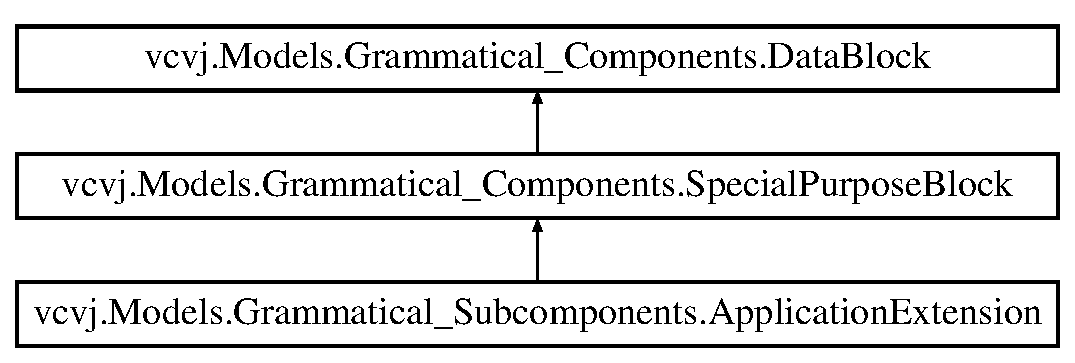
\includegraphics[height=3.000000cm]{classvcvj_1_1_models_1_1_grammatical___subcomponents_1_1_application_extension}
\end{center}
\end{figure}
\subsection*{Properties}
\begin{DoxyCompactItemize}
\item 
int {\bfseries Total\+Block\+Length}\hspace{0.3cm}{\ttfamily  \mbox{[}get, set\mbox{]}}\hypertarget{classvcvj_1_1_models_1_1_grammatical___subcomponents_1_1_application_extension_ab5cb8b441168a86a8b9368b9c91876b7}{}\label{classvcvj_1_1_models_1_1_grammatical___subcomponents_1_1_application_extension_ab5cb8b441168a86a8b9368b9c91876b7}

\item 
byte\mbox{[}$\,$\mbox{]} {\bfseries Bytes}\hspace{0.3cm}{\ttfamily  \mbox{[}get, set\mbox{]}}\hypertarget{classvcvj_1_1_models_1_1_grammatical___subcomponents_1_1_application_extension_a97f2ad5dcd13d2cde1da1817b1bcc99c}{}\label{classvcvj_1_1_models_1_1_grammatical___subcomponents_1_1_application_extension_a97f2ad5dcd13d2cde1da1817b1bcc99c}

\item 
int {\bfseries Main\+Block\+Size}\hspace{0.3cm}{\ttfamily  \mbox{[}get, set\mbox{]}}\hypertarget{classvcvj_1_1_models_1_1_grammatical___subcomponents_1_1_application_extension_ae3bec08cf62adafe9643a4ce8dd49236}{}\label{classvcvj_1_1_models_1_1_grammatical___subcomponents_1_1_application_extension_ae3bec08cf62adafe9643a4ce8dd49236}

\item 
byte\mbox{[}$\,$\mbox{]} {\bfseries Main\+Block}\hspace{0.3cm}{\ttfamily  \mbox{[}get, set\mbox{]}}\hypertarget{classvcvj_1_1_models_1_1_grammatical___subcomponents_1_1_application_extension_ad08a0a5034173cfeeeddd0f94998e59e}{}\label{classvcvj_1_1_models_1_1_grammatical___subcomponents_1_1_application_extension_ad08a0a5034173cfeeeddd0f94998e59e}

\item 
int {\bfseries Sub\+Block\+Size}\hspace{0.3cm}{\ttfamily  \mbox{[}get, set\mbox{]}}\hypertarget{classvcvj_1_1_models_1_1_grammatical___subcomponents_1_1_application_extension_ab0dd5acfa79a187d05812cfce9313015}{}\label{classvcvj_1_1_models_1_1_grammatical___subcomponents_1_1_application_extension_ab0dd5acfa79a187d05812cfce9313015}

\item 
byte\mbox{[}$\,$\mbox{]} {\bfseries Sub\+Block}\hspace{0.3cm}{\ttfamily  \mbox{[}get, set\mbox{]}}\hypertarget{classvcvj_1_1_models_1_1_grammatical___subcomponents_1_1_application_extension_a8719602be0b32fd343ac488aaeb10226}{}\label{classvcvj_1_1_models_1_1_grammatical___subcomponents_1_1_application_extension_a8719602be0b32fd343ac488aaeb10226}

\item 
string {\bfseries Application\+Identifier}\hspace{0.3cm}{\ttfamily  \mbox{[}get, set\mbox{]}}\hypertarget{classvcvj_1_1_models_1_1_grammatical___subcomponents_1_1_application_extension_a505812e93536fa6ea2f2c94706bb784b}{}\label{classvcvj_1_1_models_1_1_grammatical___subcomponents_1_1_application_extension_a505812e93536fa6ea2f2c94706bb784b}

\item 
string {\bfseries Application\+Sub\+Identifier}\hspace{0.3cm}{\ttfamily  \mbox{[}get, set\mbox{]}}\hypertarget{classvcvj_1_1_models_1_1_grammatical___subcomponents_1_1_application_extension_af1d299c56520f59f4b4c78201f9c21a6}{}\label{classvcvj_1_1_models_1_1_grammatical___subcomponents_1_1_application_extension_af1d299c56520f59f4b4c78201f9c21a6}

\end{DoxyCompactItemize}
\subsection*{Additional Inherited Members}


\subsection{Detailed Description}
An extension which contains application-\/specific instructions, including the number of times an animated G\+IF image should loop. 



The documentation for this class was generated from the following file\+:\begin{DoxyCompactItemize}
\item 
vcvj/\+Models/\+Grammatical Subcomponents/Application\+Extension.\+cs\end{DoxyCompactItemize}

\hypertarget{classvcvj_1_1_exceptions_1_1_application_extension_parser_exception}{}\section{vcvj.\+Exceptions.\+Application\+Extension\+Parser\+Exception Class Reference}
\label{classvcvj_1_1_exceptions_1_1_application_extension_parser_exception}\index{vcvj.\+Exceptions.\+Application\+Extension\+Parser\+Exception@{vcvj.\+Exceptions.\+Application\+Extension\+Parser\+Exception}}
Inheritance diagram for vcvj.\+Exceptions.\+Application\+Extension\+Parser\+Exception\+:\begin{figure}[H]
\begin{center}
\leavevmode
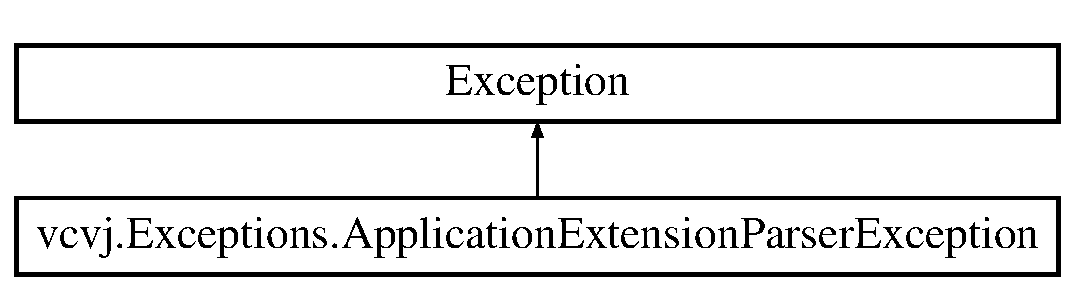
\includegraphics[height=2.000000cm]{classvcvj_1_1_exceptions_1_1_application_extension_parser_exception}
\end{center}
\end{figure}
\subsection*{Public Member Functions}
\begin{DoxyCompactItemize}
\item 
{\bfseries Application\+Extension\+Parser\+Exception} (string message)\hypertarget{classvcvj_1_1_exceptions_1_1_application_extension_parser_exception_a310bacfb7ca4f0fa4b560ef703a0d50c}{}\label{classvcvj_1_1_exceptions_1_1_application_extension_parser_exception_a310bacfb7ca4f0fa4b560ef703a0d50c}

\item 
{\bfseries Application\+Extension\+Parser\+Exception} (string message, Exception inner)\hypertarget{classvcvj_1_1_exceptions_1_1_application_extension_parser_exception_af0053eceba294b2a57801615479998d7}{}\label{classvcvj_1_1_exceptions_1_1_application_extension_parser_exception_af0053eceba294b2a57801615479998d7}

\end{DoxyCompactItemize}


The documentation for this class was generated from the following file\+:\begin{DoxyCompactItemize}
\item 
vcvj/\+Exceptions/Application\+Extension\+Parser\+Exception.\+cs\end{DoxyCompactItemize}

\hypertarget{classvcvj_1_1_models_1_1_grammatical___subcomponents_1_1_color_table}{}\section{vcvj.\+Models.\+Grammatical\+\_\+\+Subcomponents.\+Color\+Table Class Reference}
\label{classvcvj_1_1_models_1_1_grammatical___subcomponents_1_1_color_table}\index{vcvj.\+Models.\+Grammatical\+\_\+\+Subcomponents.\+Color\+Table@{vcvj.\+Models.\+Grammatical\+\_\+\+Subcomponents.\+Color\+Table}}


A block containing information about colors used. Can be global or local (frame-\/specific).  


Inheritance diagram for vcvj.\+Models.\+Grammatical\+\_\+\+Subcomponents.\+Color\+Table\+:\begin{figure}[H]
\begin{center}
\leavevmode
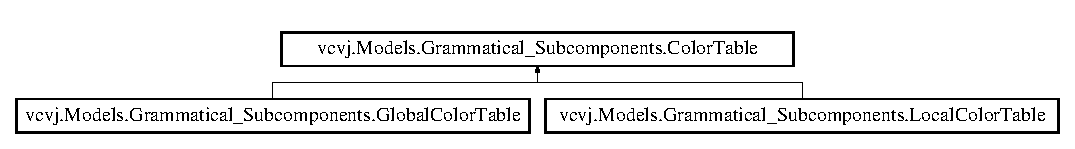
\includegraphics[height=1.555556cm]{classvcvj_1_1_models_1_1_grammatical___subcomponents_1_1_color_table}
\end{center}
\end{figure}
\subsection*{Public Member Functions}
\begin{DoxyCompactItemize}
\item 
\hyperlink{classvcvj_1_1_models_1_1_grammatical___subcomponents_1_1_color_table}{Color\+Table} \hyperlink{classvcvj_1_1_models_1_1_grammatical___subcomponents_1_1_color_table_a724c64bb00cb26222ea6c753970c9df2}{X\+OR} (byte b)
\begin{DoxyCompactList}\small\item\em X\+O\+Rs every byte in the color table with the specified byte value. \end{DoxyCompactList}\item 
\hyperlink{classvcvj_1_1_models_1_1_grammatical___subcomponents_1_1_color_table}{Color\+Table} {\bfseries Randomize} ()\hypertarget{classvcvj_1_1_models_1_1_grammatical___subcomponents_1_1_color_table_a23d1569e73caac21cfe3819afb14a7a3}{}\label{classvcvj_1_1_models_1_1_grammatical___subcomponents_1_1_color_table_a23d1569e73caac21cfe3819afb14a7a3}

\item 
\hyperlink{classvcvj_1_1_models_1_1_grammatical___subcomponents_1_1_color_table}{Color\+Table} {\bfseries Randomize\+Half} ()\hypertarget{classvcvj_1_1_models_1_1_grammatical___subcomponents_1_1_color_table_a781e9bba18f6d258e4892b0e793c9873}{}\label{classvcvj_1_1_models_1_1_grammatical___subcomponents_1_1_color_table_a781e9bba18f6d258e4892b0e793c9873}

\end{DoxyCompactItemize}
\subsection*{Properties}
\begin{DoxyCompactItemize}
\item 
byte\mbox{[}$\,$\mbox{]} {\bfseries Bytes}\hspace{0.3cm}{\ttfamily  \mbox{[}get, set\mbox{]}}\hypertarget{classvcvj_1_1_models_1_1_grammatical___subcomponents_1_1_color_table_abffe3be6aacd8aeeae897f74b1c3ac42}{}\label{classvcvj_1_1_models_1_1_grammatical___subcomponents_1_1_color_table_abffe3be6aacd8aeeae897f74b1c3ac42}

\item 
int {\bfseries Total\+Block\+Length}\hspace{0.3cm}{\ttfamily  \mbox{[}get, set\mbox{]}}\hypertarget{classvcvj_1_1_models_1_1_grammatical___subcomponents_1_1_color_table_a163f119d41d8eff30662a588bfe4719f}{}\label{classvcvj_1_1_models_1_1_grammatical___subcomponents_1_1_color_table_a163f119d41d8eff30662a588bfe4719f}

\item 
bool {\bfseries Is\+Global}\hspace{0.3cm}{\ttfamily  \mbox{[}get, set\mbox{]}}\hypertarget{classvcvj_1_1_models_1_1_grammatical___subcomponents_1_1_color_table_a85b7df61639b14b1d04379bf46756cff}{}\label{classvcvj_1_1_models_1_1_grammatical___subcomponents_1_1_color_table_a85b7df61639b14b1d04379bf46756cff}

\item 
int \hyperlink{classvcvj_1_1_models_1_1_grammatical___subcomponents_1_1_color_table_acdf650955484bc8e7b75518c5369939e}{Distinct\+Color\+Count}\hspace{0.3cm}{\ttfamily  \mbox{[}get, set\mbox{]}}
\begin{DoxyCompactList}\small\item\em The number of distinct colors in the global color table. \end{DoxyCompactList}\end{DoxyCompactItemize}


\subsection{Detailed Description}
A block containing information about colors used. Can be global or local (frame-\/specific). 



\subsection{Member Function Documentation}
\index{vcvj\+::\+Models\+::\+Grammatical\+\_\+\+Subcomponents\+::\+Color\+Table@{vcvj\+::\+Models\+::\+Grammatical\+\_\+\+Subcomponents\+::\+Color\+Table}!X\+OR@{X\+OR}}
\index{X\+OR@{X\+OR}!vcvj\+::\+Models\+::\+Grammatical\+\_\+\+Subcomponents\+::\+Color\+Table@{vcvj\+::\+Models\+::\+Grammatical\+\_\+\+Subcomponents\+::\+Color\+Table}}
\subsubsection[{\texorpdfstring{X\+O\+R(byte b)}{XOR(byte b)}}]{\setlength{\rightskip}{0pt plus 5cm}{\bf Color\+Table} vcvj.\+Models.\+Grammatical\+\_\+\+Subcomponents.\+Color\+Table.\+X\+OR (
\begin{DoxyParamCaption}
\item[{byte}]{b}
\end{DoxyParamCaption}
)\hspace{0.3cm}{\ttfamily [inline]}}\hypertarget{classvcvj_1_1_models_1_1_grammatical___subcomponents_1_1_color_table_a724c64bb00cb26222ea6c753970c9df2}{}\label{classvcvj_1_1_models_1_1_grammatical___subcomponents_1_1_color_table_a724c64bb00cb26222ea6c753970c9df2}


X\+O\+Rs every byte in the color table with the specified byte value. 

\begin{DoxyReturn}{Returns}

\end{DoxyReturn}


\subsection{Property Documentation}
\index{vcvj\+::\+Models\+::\+Grammatical\+\_\+\+Subcomponents\+::\+Color\+Table@{vcvj\+::\+Models\+::\+Grammatical\+\_\+\+Subcomponents\+::\+Color\+Table}!Distinct\+Color\+Count@{Distinct\+Color\+Count}}
\index{Distinct\+Color\+Count@{Distinct\+Color\+Count}!vcvj\+::\+Models\+::\+Grammatical\+\_\+\+Subcomponents\+::\+Color\+Table@{vcvj\+::\+Models\+::\+Grammatical\+\_\+\+Subcomponents\+::\+Color\+Table}}
\subsubsection[{\texorpdfstring{Distinct\+Color\+Count}{DistinctColorCount}}]{\setlength{\rightskip}{0pt plus 5cm}int vcvj.\+Models.\+Grammatical\+\_\+\+Subcomponents.\+Color\+Table.\+Distinct\+Color\+Count\hspace{0.3cm}{\ttfamily [get]}, {\ttfamily [set]}}\hypertarget{classvcvj_1_1_models_1_1_grammatical___subcomponents_1_1_color_table_acdf650955484bc8e7b75518c5369939e}{}\label{classvcvj_1_1_models_1_1_grammatical___subcomponents_1_1_color_table_acdf650955484bc8e7b75518c5369939e}


The number of distinct colors in the global color table. 



The documentation for this class was generated from the following file\+:\begin{DoxyCompactItemize}
\item 
vcvj/\+Models/\+Grammatical Subcomponents/Color\+Tables.\+cs\end{DoxyCompactItemize}

\hypertarget{classvcvj_1_1_models_1_1_grammatical___subcomponents_1_1_comment_extension}{}\section{vcvj.\+Models.\+Grammatical\+\_\+\+Subcomponents.\+Comment\+Extension Class Reference}
\label{classvcvj_1_1_models_1_1_grammatical___subcomponents_1_1_comment_extension}\index{vcvj.\+Models.\+Grammatical\+\_\+\+Subcomponents.\+Comment\+Extension@{vcvj.\+Models.\+Grammatical\+\_\+\+Subcomponents.\+Comment\+Extension}}


An extension containing a comment.  


Inheritance diagram for vcvj.\+Models.\+Grammatical\+\_\+\+Subcomponents.\+Comment\+Extension\+:\begin{figure}[H]
\begin{center}
\leavevmode
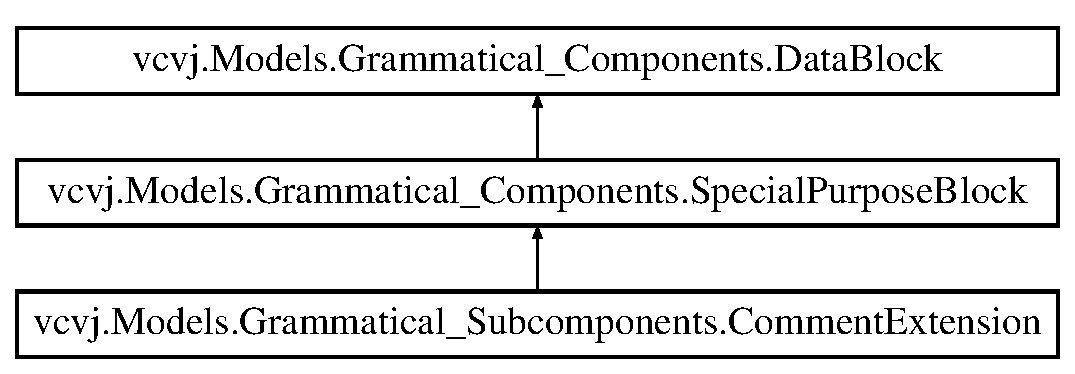
\includegraphics[height=3.000000cm]{classvcvj_1_1_models_1_1_grammatical___subcomponents_1_1_comment_extension}
\end{center}
\end{figure}
\subsection*{Properties}
\begin{DoxyCompactItemize}
\item 
byte\mbox{[}$\,$\mbox{]} {\bfseries Bytes}\hspace{0.3cm}{\ttfamily  \mbox{[}get, set\mbox{]}}\hypertarget{classvcvj_1_1_models_1_1_grammatical___subcomponents_1_1_comment_extension_a43e9e21eb429c15a5813104bae40d3eb}{}\label{classvcvj_1_1_models_1_1_grammatical___subcomponents_1_1_comment_extension_a43e9e21eb429c15a5813104bae40d3eb}

\item 
int {\bfseries Total\+Block\+Length}\hspace{0.3cm}{\ttfamily  \mbox{[}get, set\mbox{]}}\hypertarget{classvcvj_1_1_models_1_1_grammatical___subcomponents_1_1_comment_extension_a015854c766ce12c2cf5cbdabaa889e8e}{}\label{classvcvj_1_1_models_1_1_grammatical___subcomponents_1_1_comment_extension_a015854c766ce12c2cf5cbdabaa889e8e}

\item 
int {\bfseries Comment\+Length}\hspace{0.3cm}{\ttfamily  \mbox{[}get, set\mbox{]}}\hypertarget{classvcvj_1_1_models_1_1_grammatical___subcomponents_1_1_comment_extension_acbfded4d53c0101311d2c44745a80b55}{}\label{classvcvj_1_1_models_1_1_grammatical___subcomponents_1_1_comment_extension_acbfded4d53c0101311d2c44745a80b55}

\item 
string {\bfseries Comment}\hspace{0.3cm}{\ttfamily  \mbox{[}get, set\mbox{]}}\hypertarget{classvcvj_1_1_models_1_1_grammatical___subcomponents_1_1_comment_extension_a5635aba86f6c8375809715a61cc4f4d6}{}\label{classvcvj_1_1_models_1_1_grammatical___subcomponents_1_1_comment_extension_a5635aba86f6c8375809715a61cc4f4d6}

\end{DoxyCompactItemize}
\subsection*{Additional Inherited Members}


\subsection{Detailed Description}
An extension containing a comment. 



The documentation for this class was generated from the following file\+:\begin{DoxyCompactItemize}
\item 
vcvj/\+Models/\+Grammatical Subcomponents/Comment\+Extension.\+cs\end{DoxyCompactItemize}

\hypertarget{classvcvj_1_1_models_1_1_grammatical___components_1_1_data_block}{}\section{vcvj.\+Models.\+Grammatical\+\_\+\+Components.\+Data\+Block Class Reference}
\label{classvcvj_1_1_models_1_1_grammatical___components_1_1_data_block}\index{vcvj.\+Models.\+Grammatical\+\_\+\+Components.\+Data\+Block@{vcvj.\+Models.\+Grammatical\+\_\+\+Components.\+Data\+Block}}


A generic data block representing either a graphic block or a special purpose block.  


Inheritance diagram for vcvj.\+Models.\+Grammatical\+\_\+\+Components.\+Data\+Block\+:\begin{figure}[H]
\begin{center}
\leavevmode
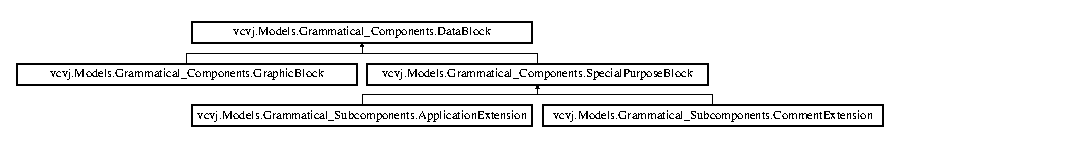
\includegraphics[height=1.477573cm]{classvcvj_1_1_models_1_1_grammatical___components_1_1_data_block}
\end{center}
\end{figure}
\subsection*{Public Member Functions}
\begin{DoxyCompactItemize}
\item 
\hyperlink{classvcvj_1_1_models_1_1_grammatical___components_1_1_graphic_block}{Graphic\+Block} \hyperlink{classvcvj_1_1_models_1_1_grammatical___components_1_1_data_block_a5ece124324f58ed9be0d0229f1d65745}{To\+Graphic\+Block} ()
\begin{DoxyCompactList}\small\item\em Casts a \hyperlink{classvcvj_1_1_models_1_1_grammatical___components_1_1_data_block}{Data\+Block} into a \hyperlink{classvcvj_1_1_models_1_1_grammatical___components_1_1_graphic_block}{Graphic\+Block}. \end{DoxyCompactList}\item 
\hyperlink{classvcvj_1_1_models_1_1_grammatical___components_1_1_special_purpose_block}{Special\+Purpose\+Block} \hyperlink{classvcvj_1_1_models_1_1_grammatical___components_1_1_data_block_ab750428e8a4df02a9c1ef7240620eeae}{To\+Special\+Purpose\+Block} ()
\begin{DoxyCompactList}\small\item\em Casts a \hyperlink{classvcvj_1_1_models_1_1_grammatical___components_1_1_data_block}{Data\+Block} into a \hyperlink{classvcvj_1_1_models_1_1_grammatical___components_1_1_special_purpose_block}{Special\+Purpose\+Block}. \end{DoxyCompactList}\item 
\hyperlink{classvcvj_1_1_models_1_1_grammatical___subcomponents_1_1_application_extension}{Application\+Extension} \hyperlink{classvcvj_1_1_models_1_1_grammatical___components_1_1_data_block_a9b92949f4970d3ffaadfaafd3b7d9640}{To\+Application\+Extension} ()
\begin{DoxyCompactList}\small\item\em Casts a \hyperlink{classvcvj_1_1_models_1_1_grammatical___components_1_1_data_block}{Data\+Block} into an Application\+Extension. \end{DoxyCompactList}\item 
\hyperlink{classvcvj_1_1_models_1_1_grammatical___subcomponents_1_1_comment_extension}{Comment\+Extension} \hyperlink{classvcvj_1_1_models_1_1_grammatical___components_1_1_data_block_a68ee3a7f3f7c0ec1b4061c1c43e09728}{To\+Comment\+Extension} ()
\begin{DoxyCompactList}\small\item\em Casts a \hyperlink{classvcvj_1_1_models_1_1_grammatical___components_1_1_data_block}{Data\+Block} into a Comment\+Extension. \end{DoxyCompactList}\item 
\hyperlink{classvcvj_1_1_models_1_1_grammatical___components_1_1_table_based_image}{Table\+Based\+Image} \hyperlink{classvcvj_1_1_models_1_1_grammatical___components_1_1_data_block_a4ac750a131443cc1e5d7ac6611b24c45}{Get\+Table\+Based\+Image} ()
\begin{DoxyCompactList}\small\item\em Gets a \hyperlink{classvcvj_1_1_models_1_1_grammatical___components_1_1_data_block}{Data\+Block}\textquotesingle{}s \hyperlink{classvcvj_1_1_models_1_1_grammatical___components_1_1_graphic_rendering_block}{Graphic\+Rendering\+Block}\textquotesingle{}s \hyperlink{classvcvj_1_1_models_1_1_grammatical___components_1_1_table_based_image}{Table\+Based\+Image}. \end{DoxyCompactList}\item 
\hyperlink{classvcvj_1_1_models_1_1_grammatical___subcomponents_1_1_plain_text_extension}{Plain\+Text\+Extension} \hyperlink{classvcvj_1_1_models_1_1_grammatical___components_1_1_data_block_a7bbaeb1dbe37e0e6770f7a84b9f35d80}{Get\+Plain\+Text\+Extension} ()
\begin{DoxyCompactList}\small\item\em Gets a \hyperlink{classvcvj_1_1_models_1_1_grammatical___components_1_1_data_block}{Data\+Block}\textquotesingle{}s \hyperlink{classvcvj_1_1_models_1_1_grammatical___components_1_1_graphic_rendering_block}{Graphic\+Rendering\+Block}\textquotesingle{}s Plain\+Text\+Extension. \end{DoxyCompactList}\end{DoxyCompactItemize}
\subsection*{Properties}
\begin{DoxyCompactItemize}
\item 
bool \hyperlink{classvcvj_1_1_models_1_1_grammatical___components_1_1_data_block_a18ed19c8e02d40cc2551f3d9dc829505}{Is\+Graphic\+Block}\hspace{0.3cm}{\ttfamily  \mbox{[}get\mbox{]}}
\begin{DoxyCompactList}\small\item\em Determines whether or not a given \hyperlink{classvcvj_1_1_models_1_1_grammatical___components_1_1_data_block}{Data\+Block} represents a \hyperlink{classvcvj_1_1_models_1_1_grammatical___components_1_1_graphic_block}{Graphic\+Block}. \end{DoxyCompactList}\item 
bool \hyperlink{classvcvj_1_1_models_1_1_grammatical___components_1_1_data_block_a734766451ecfc504f507459fffb500a8}{Is\+Special\+Purpose\+Block}\hspace{0.3cm}{\ttfamily  \mbox{[}get\mbox{]}}
\begin{DoxyCompactList}\small\item\em Determines whether or not a given \hyperlink{classvcvj_1_1_models_1_1_grammatical___components_1_1_data_block}{Data\+Block} represents a \hyperlink{classvcvj_1_1_models_1_1_grammatical___components_1_1_special_purpose_block}{Special\+Purpose\+Block}. \end{DoxyCompactList}\item 
bool \hyperlink{classvcvj_1_1_models_1_1_grammatical___components_1_1_data_block_a9bb735c2e7aa8254611cd6f0dd5af1f0}{Is\+Application\+Extension}\hspace{0.3cm}{\ttfamily  \mbox{[}get\mbox{]}}
\begin{DoxyCompactList}\small\item\em Determines whether or not a given \hyperlink{classvcvj_1_1_models_1_1_grammatical___components_1_1_data_block}{Data\+Block} represents an Application\+Extension. \end{DoxyCompactList}\item 
bool \hyperlink{classvcvj_1_1_models_1_1_grammatical___components_1_1_data_block_ad690c1a03593faeda687f872b4fa1752}{Is\+Comment\+Extension}\hspace{0.3cm}{\ttfamily  \mbox{[}get\mbox{]}}
\begin{DoxyCompactList}\small\item\em Determines whether or not a given \hyperlink{classvcvj_1_1_models_1_1_grammatical___components_1_1_data_block}{Data\+Block} represents a Comment\+Extension. \end{DoxyCompactList}\item 
bool \hyperlink{classvcvj_1_1_models_1_1_grammatical___components_1_1_data_block_a5e1cede8610e08ba960710f5e5bf1293}{Has\+Table\+Based\+Image}\hspace{0.3cm}{\ttfamily  \mbox{[}get\mbox{]}}
\begin{DoxyCompactList}\small\item\em Determines whether or not a given \hyperlink{classvcvj_1_1_models_1_1_grammatical___components_1_1_data_block}{Data\+Block} represents a \hyperlink{classvcvj_1_1_models_1_1_grammatical___components_1_1_graphic_block}{Graphic\+Block}, whose \hyperlink{classvcvj_1_1_models_1_1_grammatical___components_1_1_graphic_rendering_block}{Graphic\+Rendering\+Block} represents a \hyperlink{classvcvj_1_1_models_1_1_grammatical___components_1_1_table_based_image}{Table\+Based\+Image}. \end{DoxyCompactList}\item 
bool \hyperlink{classvcvj_1_1_models_1_1_grammatical___components_1_1_data_block_a6d08fab7e1c1ba82f00f220655f6aa9b}{Has\+Plain\+Text\+Extension}\hspace{0.3cm}{\ttfamily  \mbox{[}get\mbox{]}}
\begin{DoxyCompactList}\small\item\em Determines whether or not a given \hyperlink{classvcvj_1_1_models_1_1_grammatical___components_1_1_data_block}{Data\+Block} represents a \hyperlink{classvcvj_1_1_models_1_1_grammatical___components_1_1_graphic_block}{Graphic\+Block}, whose \hyperlink{classvcvj_1_1_models_1_1_grammatical___components_1_1_graphic_rendering_block}{Graphic\+Rendering\+Block} represents a Plain\+Text\+Extension. \end{DoxyCompactList}\end{DoxyCompactItemize}


\subsection{Detailed Description}
A generic data block representing either a graphic block or a special purpose block. 



\subsection{Member Function Documentation}
\index{vcvj\+::\+Models\+::\+Grammatical\+\_\+\+Components\+::\+Data\+Block@{vcvj\+::\+Models\+::\+Grammatical\+\_\+\+Components\+::\+Data\+Block}!Get\+Plain\+Text\+Extension@{Get\+Plain\+Text\+Extension}}
\index{Get\+Plain\+Text\+Extension@{Get\+Plain\+Text\+Extension}!vcvj\+::\+Models\+::\+Grammatical\+\_\+\+Components\+::\+Data\+Block@{vcvj\+::\+Models\+::\+Grammatical\+\_\+\+Components\+::\+Data\+Block}}
\subsubsection[{\texorpdfstring{Get\+Plain\+Text\+Extension()}{GetPlainTextExtension()}}]{\setlength{\rightskip}{0pt plus 5cm}{\bf Plain\+Text\+Extension} vcvj.\+Models.\+Grammatical\+\_\+\+Components.\+Data\+Block.\+Get\+Plain\+Text\+Extension (
\begin{DoxyParamCaption}
{}
\end{DoxyParamCaption}
)\hspace{0.3cm}{\ttfamily [inline]}}\hypertarget{classvcvj_1_1_models_1_1_grammatical___components_1_1_data_block_a7bbaeb1dbe37e0e6770f7a84b9f35d80}{}\label{classvcvj_1_1_models_1_1_grammatical___components_1_1_data_block_a7bbaeb1dbe37e0e6770f7a84b9f35d80}


Gets a \hyperlink{classvcvj_1_1_models_1_1_grammatical___components_1_1_data_block}{Data\+Block}\textquotesingle{}s \hyperlink{classvcvj_1_1_models_1_1_grammatical___components_1_1_graphic_rendering_block}{Graphic\+Rendering\+Block}\textquotesingle{}s Plain\+Text\+Extension. 

\index{vcvj\+::\+Models\+::\+Grammatical\+\_\+\+Components\+::\+Data\+Block@{vcvj\+::\+Models\+::\+Grammatical\+\_\+\+Components\+::\+Data\+Block}!Get\+Table\+Based\+Image@{Get\+Table\+Based\+Image}}
\index{Get\+Table\+Based\+Image@{Get\+Table\+Based\+Image}!vcvj\+::\+Models\+::\+Grammatical\+\_\+\+Components\+::\+Data\+Block@{vcvj\+::\+Models\+::\+Grammatical\+\_\+\+Components\+::\+Data\+Block}}
\subsubsection[{\texorpdfstring{Get\+Table\+Based\+Image()}{GetTableBasedImage()}}]{\setlength{\rightskip}{0pt plus 5cm}{\bf Table\+Based\+Image} vcvj.\+Models.\+Grammatical\+\_\+\+Components.\+Data\+Block.\+Get\+Table\+Based\+Image (
\begin{DoxyParamCaption}
{}
\end{DoxyParamCaption}
)\hspace{0.3cm}{\ttfamily [inline]}}\hypertarget{classvcvj_1_1_models_1_1_grammatical___components_1_1_data_block_a4ac750a131443cc1e5d7ac6611b24c45}{}\label{classvcvj_1_1_models_1_1_grammatical___components_1_1_data_block_a4ac750a131443cc1e5d7ac6611b24c45}


Gets a \hyperlink{classvcvj_1_1_models_1_1_grammatical___components_1_1_data_block}{Data\+Block}\textquotesingle{}s \hyperlink{classvcvj_1_1_models_1_1_grammatical___components_1_1_graphic_rendering_block}{Graphic\+Rendering\+Block}\textquotesingle{}s \hyperlink{classvcvj_1_1_models_1_1_grammatical___components_1_1_table_based_image}{Table\+Based\+Image}. 

\index{vcvj\+::\+Models\+::\+Grammatical\+\_\+\+Components\+::\+Data\+Block@{vcvj\+::\+Models\+::\+Grammatical\+\_\+\+Components\+::\+Data\+Block}!To\+Application\+Extension@{To\+Application\+Extension}}
\index{To\+Application\+Extension@{To\+Application\+Extension}!vcvj\+::\+Models\+::\+Grammatical\+\_\+\+Components\+::\+Data\+Block@{vcvj\+::\+Models\+::\+Grammatical\+\_\+\+Components\+::\+Data\+Block}}
\subsubsection[{\texorpdfstring{To\+Application\+Extension()}{ToApplicationExtension()}}]{\setlength{\rightskip}{0pt plus 5cm}{\bf Application\+Extension} vcvj.\+Models.\+Grammatical\+\_\+\+Components.\+Data\+Block.\+To\+Application\+Extension (
\begin{DoxyParamCaption}
{}
\end{DoxyParamCaption}
)\hspace{0.3cm}{\ttfamily [inline]}}\hypertarget{classvcvj_1_1_models_1_1_grammatical___components_1_1_data_block_a9b92949f4970d3ffaadfaafd3b7d9640}{}\label{classvcvj_1_1_models_1_1_grammatical___components_1_1_data_block_a9b92949f4970d3ffaadfaafd3b7d9640}


Casts a \hyperlink{classvcvj_1_1_models_1_1_grammatical___components_1_1_data_block}{Data\+Block} into an Application\+Extension. 

\index{vcvj\+::\+Models\+::\+Grammatical\+\_\+\+Components\+::\+Data\+Block@{vcvj\+::\+Models\+::\+Grammatical\+\_\+\+Components\+::\+Data\+Block}!To\+Comment\+Extension@{To\+Comment\+Extension}}
\index{To\+Comment\+Extension@{To\+Comment\+Extension}!vcvj\+::\+Models\+::\+Grammatical\+\_\+\+Components\+::\+Data\+Block@{vcvj\+::\+Models\+::\+Grammatical\+\_\+\+Components\+::\+Data\+Block}}
\subsubsection[{\texorpdfstring{To\+Comment\+Extension()}{ToCommentExtension()}}]{\setlength{\rightskip}{0pt plus 5cm}{\bf Comment\+Extension} vcvj.\+Models.\+Grammatical\+\_\+\+Components.\+Data\+Block.\+To\+Comment\+Extension (
\begin{DoxyParamCaption}
{}
\end{DoxyParamCaption}
)\hspace{0.3cm}{\ttfamily [inline]}}\hypertarget{classvcvj_1_1_models_1_1_grammatical___components_1_1_data_block_a68ee3a7f3f7c0ec1b4061c1c43e09728}{}\label{classvcvj_1_1_models_1_1_grammatical___components_1_1_data_block_a68ee3a7f3f7c0ec1b4061c1c43e09728}


Casts a \hyperlink{classvcvj_1_1_models_1_1_grammatical___components_1_1_data_block}{Data\+Block} into a Comment\+Extension. 

\index{vcvj\+::\+Models\+::\+Grammatical\+\_\+\+Components\+::\+Data\+Block@{vcvj\+::\+Models\+::\+Grammatical\+\_\+\+Components\+::\+Data\+Block}!To\+Graphic\+Block@{To\+Graphic\+Block}}
\index{To\+Graphic\+Block@{To\+Graphic\+Block}!vcvj\+::\+Models\+::\+Grammatical\+\_\+\+Components\+::\+Data\+Block@{vcvj\+::\+Models\+::\+Grammatical\+\_\+\+Components\+::\+Data\+Block}}
\subsubsection[{\texorpdfstring{To\+Graphic\+Block()}{ToGraphicBlock()}}]{\setlength{\rightskip}{0pt plus 5cm}{\bf Graphic\+Block} vcvj.\+Models.\+Grammatical\+\_\+\+Components.\+Data\+Block.\+To\+Graphic\+Block (
\begin{DoxyParamCaption}
{}
\end{DoxyParamCaption}
)\hspace{0.3cm}{\ttfamily [inline]}}\hypertarget{classvcvj_1_1_models_1_1_grammatical___components_1_1_data_block_a5ece124324f58ed9be0d0229f1d65745}{}\label{classvcvj_1_1_models_1_1_grammatical___components_1_1_data_block_a5ece124324f58ed9be0d0229f1d65745}


Casts a \hyperlink{classvcvj_1_1_models_1_1_grammatical___components_1_1_data_block}{Data\+Block} into a \hyperlink{classvcvj_1_1_models_1_1_grammatical___components_1_1_graphic_block}{Graphic\+Block}. 

\index{vcvj\+::\+Models\+::\+Grammatical\+\_\+\+Components\+::\+Data\+Block@{vcvj\+::\+Models\+::\+Grammatical\+\_\+\+Components\+::\+Data\+Block}!To\+Special\+Purpose\+Block@{To\+Special\+Purpose\+Block}}
\index{To\+Special\+Purpose\+Block@{To\+Special\+Purpose\+Block}!vcvj\+::\+Models\+::\+Grammatical\+\_\+\+Components\+::\+Data\+Block@{vcvj\+::\+Models\+::\+Grammatical\+\_\+\+Components\+::\+Data\+Block}}
\subsubsection[{\texorpdfstring{To\+Special\+Purpose\+Block()}{ToSpecialPurposeBlock()}}]{\setlength{\rightskip}{0pt plus 5cm}{\bf Special\+Purpose\+Block} vcvj.\+Models.\+Grammatical\+\_\+\+Components.\+Data\+Block.\+To\+Special\+Purpose\+Block (
\begin{DoxyParamCaption}
{}
\end{DoxyParamCaption}
)\hspace{0.3cm}{\ttfamily [inline]}}\hypertarget{classvcvj_1_1_models_1_1_grammatical___components_1_1_data_block_ab750428e8a4df02a9c1ef7240620eeae}{}\label{classvcvj_1_1_models_1_1_grammatical___components_1_1_data_block_ab750428e8a4df02a9c1ef7240620eeae}


Casts a \hyperlink{classvcvj_1_1_models_1_1_grammatical___components_1_1_data_block}{Data\+Block} into a \hyperlink{classvcvj_1_1_models_1_1_grammatical___components_1_1_special_purpose_block}{Special\+Purpose\+Block}. 



\subsection{Property Documentation}
\index{vcvj\+::\+Models\+::\+Grammatical\+\_\+\+Components\+::\+Data\+Block@{vcvj\+::\+Models\+::\+Grammatical\+\_\+\+Components\+::\+Data\+Block}!Has\+Plain\+Text\+Extension@{Has\+Plain\+Text\+Extension}}
\index{Has\+Plain\+Text\+Extension@{Has\+Plain\+Text\+Extension}!vcvj\+::\+Models\+::\+Grammatical\+\_\+\+Components\+::\+Data\+Block@{vcvj\+::\+Models\+::\+Grammatical\+\_\+\+Components\+::\+Data\+Block}}
\subsubsection[{\texorpdfstring{Has\+Plain\+Text\+Extension}{HasPlainTextExtension}}]{\setlength{\rightskip}{0pt plus 5cm}bool vcvj.\+Models.\+Grammatical\+\_\+\+Components.\+Data\+Block.\+Has\+Plain\+Text\+Extension\hspace{0.3cm}{\ttfamily [get]}}\hypertarget{classvcvj_1_1_models_1_1_grammatical___components_1_1_data_block_a6d08fab7e1c1ba82f00f220655f6aa9b}{}\label{classvcvj_1_1_models_1_1_grammatical___components_1_1_data_block_a6d08fab7e1c1ba82f00f220655f6aa9b}


Determines whether or not a given \hyperlink{classvcvj_1_1_models_1_1_grammatical___components_1_1_data_block}{Data\+Block} represents a \hyperlink{classvcvj_1_1_models_1_1_grammatical___components_1_1_graphic_block}{Graphic\+Block}, whose \hyperlink{classvcvj_1_1_models_1_1_grammatical___components_1_1_graphic_rendering_block}{Graphic\+Rendering\+Block} represents a Plain\+Text\+Extension. 

\index{vcvj\+::\+Models\+::\+Grammatical\+\_\+\+Components\+::\+Data\+Block@{vcvj\+::\+Models\+::\+Grammatical\+\_\+\+Components\+::\+Data\+Block}!Has\+Table\+Based\+Image@{Has\+Table\+Based\+Image}}
\index{Has\+Table\+Based\+Image@{Has\+Table\+Based\+Image}!vcvj\+::\+Models\+::\+Grammatical\+\_\+\+Components\+::\+Data\+Block@{vcvj\+::\+Models\+::\+Grammatical\+\_\+\+Components\+::\+Data\+Block}}
\subsubsection[{\texorpdfstring{Has\+Table\+Based\+Image}{HasTableBasedImage}}]{\setlength{\rightskip}{0pt plus 5cm}bool vcvj.\+Models.\+Grammatical\+\_\+\+Components.\+Data\+Block.\+Has\+Table\+Based\+Image\hspace{0.3cm}{\ttfamily [get]}}\hypertarget{classvcvj_1_1_models_1_1_grammatical___components_1_1_data_block_a5e1cede8610e08ba960710f5e5bf1293}{}\label{classvcvj_1_1_models_1_1_grammatical___components_1_1_data_block_a5e1cede8610e08ba960710f5e5bf1293}


Determines whether or not a given \hyperlink{classvcvj_1_1_models_1_1_grammatical___components_1_1_data_block}{Data\+Block} represents a \hyperlink{classvcvj_1_1_models_1_1_grammatical___components_1_1_graphic_block}{Graphic\+Block}, whose \hyperlink{classvcvj_1_1_models_1_1_grammatical___components_1_1_graphic_rendering_block}{Graphic\+Rendering\+Block} represents a \hyperlink{classvcvj_1_1_models_1_1_grammatical___components_1_1_table_based_image}{Table\+Based\+Image}. 

\index{vcvj\+::\+Models\+::\+Grammatical\+\_\+\+Components\+::\+Data\+Block@{vcvj\+::\+Models\+::\+Grammatical\+\_\+\+Components\+::\+Data\+Block}!Is\+Application\+Extension@{Is\+Application\+Extension}}
\index{Is\+Application\+Extension@{Is\+Application\+Extension}!vcvj\+::\+Models\+::\+Grammatical\+\_\+\+Components\+::\+Data\+Block@{vcvj\+::\+Models\+::\+Grammatical\+\_\+\+Components\+::\+Data\+Block}}
\subsubsection[{\texorpdfstring{Is\+Application\+Extension}{IsApplicationExtension}}]{\setlength{\rightskip}{0pt plus 5cm}bool vcvj.\+Models.\+Grammatical\+\_\+\+Components.\+Data\+Block.\+Is\+Application\+Extension\hspace{0.3cm}{\ttfamily [get]}}\hypertarget{classvcvj_1_1_models_1_1_grammatical___components_1_1_data_block_a9bb735c2e7aa8254611cd6f0dd5af1f0}{}\label{classvcvj_1_1_models_1_1_grammatical___components_1_1_data_block_a9bb735c2e7aa8254611cd6f0dd5af1f0}


Determines whether or not a given \hyperlink{classvcvj_1_1_models_1_1_grammatical___components_1_1_data_block}{Data\+Block} represents an Application\+Extension. 

\index{vcvj\+::\+Models\+::\+Grammatical\+\_\+\+Components\+::\+Data\+Block@{vcvj\+::\+Models\+::\+Grammatical\+\_\+\+Components\+::\+Data\+Block}!Is\+Comment\+Extension@{Is\+Comment\+Extension}}
\index{Is\+Comment\+Extension@{Is\+Comment\+Extension}!vcvj\+::\+Models\+::\+Grammatical\+\_\+\+Components\+::\+Data\+Block@{vcvj\+::\+Models\+::\+Grammatical\+\_\+\+Components\+::\+Data\+Block}}
\subsubsection[{\texorpdfstring{Is\+Comment\+Extension}{IsCommentExtension}}]{\setlength{\rightskip}{0pt plus 5cm}bool vcvj.\+Models.\+Grammatical\+\_\+\+Components.\+Data\+Block.\+Is\+Comment\+Extension\hspace{0.3cm}{\ttfamily [get]}}\hypertarget{classvcvj_1_1_models_1_1_grammatical___components_1_1_data_block_ad690c1a03593faeda687f872b4fa1752}{}\label{classvcvj_1_1_models_1_1_grammatical___components_1_1_data_block_ad690c1a03593faeda687f872b4fa1752}


Determines whether or not a given \hyperlink{classvcvj_1_1_models_1_1_grammatical___components_1_1_data_block}{Data\+Block} represents a Comment\+Extension. 

\index{vcvj\+::\+Models\+::\+Grammatical\+\_\+\+Components\+::\+Data\+Block@{vcvj\+::\+Models\+::\+Grammatical\+\_\+\+Components\+::\+Data\+Block}!Is\+Graphic\+Block@{Is\+Graphic\+Block}}
\index{Is\+Graphic\+Block@{Is\+Graphic\+Block}!vcvj\+::\+Models\+::\+Grammatical\+\_\+\+Components\+::\+Data\+Block@{vcvj\+::\+Models\+::\+Grammatical\+\_\+\+Components\+::\+Data\+Block}}
\subsubsection[{\texorpdfstring{Is\+Graphic\+Block}{IsGraphicBlock}}]{\setlength{\rightskip}{0pt plus 5cm}bool vcvj.\+Models.\+Grammatical\+\_\+\+Components.\+Data\+Block.\+Is\+Graphic\+Block\hspace{0.3cm}{\ttfamily [get]}}\hypertarget{classvcvj_1_1_models_1_1_grammatical___components_1_1_data_block_a18ed19c8e02d40cc2551f3d9dc829505}{}\label{classvcvj_1_1_models_1_1_grammatical___components_1_1_data_block_a18ed19c8e02d40cc2551f3d9dc829505}


Determines whether or not a given \hyperlink{classvcvj_1_1_models_1_1_grammatical___components_1_1_data_block}{Data\+Block} represents a \hyperlink{classvcvj_1_1_models_1_1_grammatical___components_1_1_graphic_block}{Graphic\+Block}. 

\index{vcvj\+::\+Models\+::\+Grammatical\+\_\+\+Components\+::\+Data\+Block@{vcvj\+::\+Models\+::\+Grammatical\+\_\+\+Components\+::\+Data\+Block}!Is\+Special\+Purpose\+Block@{Is\+Special\+Purpose\+Block}}
\index{Is\+Special\+Purpose\+Block@{Is\+Special\+Purpose\+Block}!vcvj\+::\+Models\+::\+Grammatical\+\_\+\+Components\+::\+Data\+Block@{vcvj\+::\+Models\+::\+Grammatical\+\_\+\+Components\+::\+Data\+Block}}
\subsubsection[{\texorpdfstring{Is\+Special\+Purpose\+Block}{IsSpecialPurposeBlock}}]{\setlength{\rightskip}{0pt plus 5cm}bool vcvj.\+Models.\+Grammatical\+\_\+\+Components.\+Data\+Block.\+Is\+Special\+Purpose\+Block\hspace{0.3cm}{\ttfamily [get]}}\hypertarget{classvcvj_1_1_models_1_1_grammatical___components_1_1_data_block_a734766451ecfc504f507459fffb500a8}{}\label{classvcvj_1_1_models_1_1_grammatical___components_1_1_data_block_a734766451ecfc504f507459fffb500a8}


Determines whether or not a given \hyperlink{classvcvj_1_1_models_1_1_grammatical___components_1_1_data_block}{Data\+Block} represents a \hyperlink{classvcvj_1_1_models_1_1_grammatical___components_1_1_special_purpose_block}{Special\+Purpose\+Block}. 



The documentation for this class was generated from the following file\+:\begin{DoxyCompactItemize}
\item 
vcvj/\+Models/\+Grammatical Components/Data\+Block.\+cs\end{DoxyCompactItemize}

\hypertarget{classvcvj_1_1_models_1_1_grammatical___components_1_1_data_stream}{}\section{vcvj.\+Models.\+Grammatical\+\_\+\+Components.\+Data\+Stream Class Reference}
\label{classvcvj_1_1_models_1_1_grammatical___components_1_1_data_stream}\index{vcvj.\+Models.\+Grammatical\+\_\+\+Components.\+Data\+Stream@{vcvj.\+Models.\+Grammatical\+\_\+\+Components.\+Data\+Stream}}
\subsection*{Public Member Functions}
\begin{DoxyCompactItemize}
\item 
int \hyperlink{classvcvj_1_1_models_1_1_grammatical___components_1_1_data_stream_ad3cefa460a8e8766862279a17355b402}{Get\+Length} ()
\begin{DoxyCompactList}\small\item\em Returns the length of the parsed data stream byte\mbox{[}\mbox{]}. \end{DoxyCompactList}\item 
List$<$ \hyperlink{classvcvj_1_1_models_1_1_grammatical___components_1_1_table_based_image}{Table\+Based\+Image} $>$ \hyperlink{classvcvj_1_1_models_1_1_grammatical___components_1_1_data_stream_a0afb27b16b52529ef68cd5095e074971}{Get\+Table\+Based\+Images} ()
\begin{DoxyCompactList}\small\item\em Returns a list of Table\+Base\+Images in the data stream. \end{DoxyCompactList}\item 
\hyperlink{classvcvj_1_1_models_1_1_grammatical___components_1_1_data_stream}{Data\+Stream} \hyperlink{classvcvj_1_1_models_1_1_grammatical___components_1_1_data_stream_a7df0fc648d33803779668e00720379d6}{Randomize\+Frames} ()
\begin{DoxyCompactList}\small\item\em Randomizes the frames of the data stream. \end{DoxyCompactList}\item 
\hyperlink{classvcvj_1_1_models_1_1_grammatical___components_1_1_data_stream}{Data\+Stream} \hyperlink{classvcvj_1_1_models_1_1_grammatical___components_1_1_data_stream_a0d6571ea9e0fc3d983e003b79266130a}{Reverse\+Data\+Blocks} ()
\begin{DoxyCompactList}\small\item\em Reverses the order of Data\+Blocks in the data stream. \end{DoxyCompactList}\item 
\hyperlink{classvcvj_1_1_models_1_1_grammatical___components_1_1_data_stream}{Data\+Stream} \hyperlink{classvcvj_1_1_models_1_1_grammatical___components_1_1_data_stream_acc25a5965b38129773a783f6f73531d0}{Reverse\+Frames} ()
\begin{DoxyCompactList}\small\item\em Reverses the order of the frames in the data stream. \end{DoxyCompactList}\item 
\hyperlink{classvcvj_1_1_models_1_1_grammatical___components_1_1_data_stream}{Data\+Stream} \hyperlink{classvcvj_1_1_models_1_1_grammatical___components_1_1_data_stream_a5b0888f317857e784b4bc54f9d3b6a0f}{Delete\+Chunks} (int chunk\+Length)
\begin{DoxyCompactList}\small\item\em Deletes random data from the compiled byte array. \end{DoxyCompactList}\end{DoxyCompactItemize}
\subsection*{Public Attributes}
\begin{DoxyCompactItemize}
\item 
\hyperlink{classvcvj_1_1_models_1_1_grammatical___subcomponents_1_1_header}{Header} {\bfseries Header} = new \hyperlink{classvcvj_1_1_models_1_1_grammatical___subcomponents_1_1_header}{Header}()\hypertarget{classvcvj_1_1_models_1_1_grammatical___components_1_1_data_stream_a92d5f935a37800ae38fbc9a7f084f833}{}\label{classvcvj_1_1_models_1_1_grammatical___components_1_1_data_stream_a92d5f935a37800ae38fbc9a7f084f833}

\item 
\hyperlink{classvcvj_1_1_models_1_1_grammatical___components_1_1_logical_screen}{Logical\+Screen} {\bfseries Logical\+Screen} = new \hyperlink{classvcvj_1_1_models_1_1_grammatical___components_1_1_logical_screen}{Logical\+Screen}()\hypertarget{classvcvj_1_1_models_1_1_grammatical___components_1_1_data_stream_a3bf3a2c2d59f08902e885630f7753cc6}{}\label{classvcvj_1_1_models_1_1_grammatical___components_1_1_data_stream_a3bf3a2c2d59f08902e885630f7753cc6}

\item 
List$<$ \hyperlink{classvcvj_1_1_models_1_1_grammatical___components_1_1_data_block}{Data\+Block} $>$ {\bfseries Data\+Blocks} = new List$<$\hyperlink{classvcvj_1_1_models_1_1_grammatical___components_1_1_data_block}{Data\+Block}$>$()\hypertarget{classvcvj_1_1_models_1_1_grammatical___components_1_1_data_stream_aef30dc520b3cd5bdaa923cd38523ebe8}{}\label{classvcvj_1_1_models_1_1_grammatical___components_1_1_data_stream_aef30dc520b3cd5bdaa923cd38523ebe8}

\item 
\hyperlink{classvcvj_1_1_models_1_1_grammatical___subcomponents_1_1_trailer}{Trailer} {\bfseries Trailer} = new \hyperlink{classvcvj_1_1_models_1_1_grammatical___subcomponents_1_1_trailer}{Trailer}()\hypertarget{classvcvj_1_1_models_1_1_grammatical___components_1_1_data_stream_ab4ab89e961946602546c555e89c23d74}{}\label{classvcvj_1_1_models_1_1_grammatical___components_1_1_data_stream_ab4ab89e961946602546c555e89c23d74}

\end{DoxyCompactItemize}
\subsection*{Properties}
\begin{DoxyCompactItemize}
\item 
int {\bfseries Data\+Blocks\+Starting\+Index}\hspace{0.3cm}{\ttfamily  \mbox{[}get\mbox{]}}\hypertarget{classvcvj_1_1_models_1_1_grammatical___components_1_1_data_stream_ab2ee0c6e93b8da07d63ab701ec8ab2d5}{}\label{classvcvj_1_1_models_1_1_grammatical___components_1_1_data_stream_ab2ee0c6e93b8da07d63ab701ec8ab2d5}

\item 
byte\mbox{[}$\,$\mbox{]} {\bfseries Bytes}\hspace{0.3cm}{\ttfamily  \mbox{[}get, set\mbox{]}}\hypertarget{classvcvj_1_1_models_1_1_grammatical___components_1_1_data_stream_a4ce8dd14c1c17dc606b6a272d7b6fef6}{}\label{classvcvj_1_1_models_1_1_grammatical___components_1_1_data_stream_a4ce8dd14c1c17dc606b6a272d7b6fef6}

\end{DoxyCompactItemize}


\subsection{Member Function Documentation}
\index{vcvj\+::\+Models\+::\+Grammatical\+\_\+\+Components\+::\+Data\+Stream@{vcvj\+::\+Models\+::\+Grammatical\+\_\+\+Components\+::\+Data\+Stream}!Delete\+Chunks@{Delete\+Chunks}}
\index{Delete\+Chunks@{Delete\+Chunks}!vcvj\+::\+Models\+::\+Grammatical\+\_\+\+Components\+::\+Data\+Stream@{vcvj\+::\+Models\+::\+Grammatical\+\_\+\+Components\+::\+Data\+Stream}}
\subsubsection[{\texorpdfstring{Delete\+Chunks(int chunk\+Length)}{DeleteChunks(int chunkLength)}}]{\setlength{\rightskip}{0pt plus 5cm}{\bf Data\+Stream} vcvj.\+Models.\+Grammatical\+\_\+\+Components.\+Data\+Stream.\+Delete\+Chunks (
\begin{DoxyParamCaption}
\item[{int}]{chunk\+Length}
\end{DoxyParamCaption}
)\hspace{0.3cm}{\ttfamily [inline]}}\hypertarget{classvcvj_1_1_models_1_1_grammatical___components_1_1_data_stream_a5b0888f317857e784b4bc54f9d3b6a0f}{}\label{classvcvj_1_1_models_1_1_grammatical___components_1_1_data_stream_a5b0888f317857e784b4bc54f9d3b6a0f}


Deletes random data from the compiled byte array. 


\begin{DoxyParams}{Parameters}
{\em chunk\+Length} & \\
\hline
\end{DoxyParams}
\begin{DoxyReturn}{Returns}

\end{DoxyReturn}
\index{vcvj\+::\+Models\+::\+Grammatical\+\_\+\+Components\+::\+Data\+Stream@{vcvj\+::\+Models\+::\+Grammatical\+\_\+\+Components\+::\+Data\+Stream}!Get\+Length@{Get\+Length}}
\index{Get\+Length@{Get\+Length}!vcvj\+::\+Models\+::\+Grammatical\+\_\+\+Components\+::\+Data\+Stream@{vcvj\+::\+Models\+::\+Grammatical\+\_\+\+Components\+::\+Data\+Stream}}
\subsubsection[{\texorpdfstring{Get\+Length()}{GetLength()}}]{\setlength{\rightskip}{0pt plus 5cm}int vcvj.\+Models.\+Grammatical\+\_\+\+Components.\+Data\+Stream.\+Get\+Length (
\begin{DoxyParamCaption}
{}
\end{DoxyParamCaption}
)\hspace{0.3cm}{\ttfamily [inline]}}\hypertarget{classvcvj_1_1_models_1_1_grammatical___components_1_1_data_stream_ad3cefa460a8e8766862279a17355b402}{}\label{classvcvj_1_1_models_1_1_grammatical___components_1_1_data_stream_ad3cefa460a8e8766862279a17355b402}


Returns the length of the parsed data stream byte\mbox{[}\mbox{]}. 

\begin{DoxyReturn}{Returns}

\end{DoxyReturn}
\index{vcvj\+::\+Models\+::\+Grammatical\+\_\+\+Components\+::\+Data\+Stream@{vcvj\+::\+Models\+::\+Grammatical\+\_\+\+Components\+::\+Data\+Stream}!Get\+Table\+Based\+Images@{Get\+Table\+Based\+Images}}
\index{Get\+Table\+Based\+Images@{Get\+Table\+Based\+Images}!vcvj\+::\+Models\+::\+Grammatical\+\_\+\+Components\+::\+Data\+Stream@{vcvj\+::\+Models\+::\+Grammatical\+\_\+\+Components\+::\+Data\+Stream}}
\subsubsection[{\texorpdfstring{Get\+Table\+Based\+Images()}{GetTableBasedImages()}}]{\setlength{\rightskip}{0pt plus 5cm}List$<${\bf Table\+Based\+Image}$>$ vcvj.\+Models.\+Grammatical\+\_\+\+Components.\+Data\+Stream.\+Get\+Table\+Based\+Images (
\begin{DoxyParamCaption}
{}
\end{DoxyParamCaption}
)\hspace{0.3cm}{\ttfamily [inline]}}\hypertarget{classvcvj_1_1_models_1_1_grammatical___components_1_1_data_stream_a0afb27b16b52529ef68cd5095e074971}{}\label{classvcvj_1_1_models_1_1_grammatical___components_1_1_data_stream_a0afb27b16b52529ef68cd5095e074971}


Returns a list of Table\+Base\+Images in the data stream. 

\begin{DoxyReturn}{Returns}

\end{DoxyReturn}
\index{vcvj\+::\+Models\+::\+Grammatical\+\_\+\+Components\+::\+Data\+Stream@{vcvj\+::\+Models\+::\+Grammatical\+\_\+\+Components\+::\+Data\+Stream}!Randomize\+Frames@{Randomize\+Frames}}
\index{Randomize\+Frames@{Randomize\+Frames}!vcvj\+::\+Models\+::\+Grammatical\+\_\+\+Components\+::\+Data\+Stream@{vcvj\+::\+Models\+::\+Grammatical\+\_\+\+Components\+::\+Data\+Stream}}
\subsubsection[{\texorpdfstring{Randomize\+Frames()}{RandomizeFrames()}}]{\setlength{\rightskip}{0pt plus 5cm}{\bf Data\+Stream} vcvj.\+Models.\+Grammatical\+\_\+\+Components.\+Data\+Stream.\+Randomize\+Frames (
\begin{DoxyParamCaption}
{}
\end{DoxyParamCaption}
)\hspace{0.3cm}{\ttfamily [inline]}}\hypertarget{classvcvj_1_1_models_1_1_grammatical___components_1_1_data_stream_a7df0fc648d33803779668e00720379d6}{}\label{classvcvj_1_1_models_1_1_grammatical___components_1_1_data_stream_a7df0fc648d33803779668e00720379d6}


Randomizes the frames of the data stream. 

\begin{DoxyReturn}{Returns}

\end{DoxyReturn}
\index{vcvj\+::\+Models\+::\+Grammatical\+\_\+\+Components\+::\+Data\+Stream@{vcvj\+::\+Models\+::\+Grammatical\+\_\+\+Components\+::\+Data\+Stream}!Reverse\+Data\+Blocks@{Reverse\+Data\+Blocks}}
\index{Reverse\+Data\+Blocks@{Reverse\+Data\+Blocks}!vcvj\+::\+Models\+::\+Grammatical\+\_\+\+Components\+::\+Data\+Stream@{vcvj\+::\+Models\+::\+Grammatical\+\_\+\+Components\+::\+Data\+Stream}}
\subsubsection[{\texorpdfstring{Reverse\+Data\+Blocks()}{ReverseDataBlocks()}}]{\setlength{\rightskip}{0pt plus 5cm}{\bf Data\+Stream} vcvj.\+Models.\+Grammatical\+\_\+\+Components.\+Data\+Stream.\+Reverse\+Data\+Blocks (
\begin{DoxyParamCaption}
{}
\end{DoxyParamCaption}
)\hspace{0.3cm}{\ttfamily [inline]}}\hypertarget{classvcvj_1_1_models_1_1_grammatical___components_1_1_data_stream_a0d6571ea9e0fc3d983e003b79266130a}{}\label{classvcvj_1_1_models_1_1_grammatical___components_1_1_data_stream_a0d6571ea9e0fc3d983e003b79266130a}


Reverses the order of Data\+Blocks in the data stream. 

\begin{DoxyReturn}{Returns}

\end{DoxyReturn}
\index{vcvj\+::\+Models\+::\+Grammatical\+\_\+\+Components\+::\+Data\+Stream@{vcvj\+::\+Models\+::\+Grammatical\+\_\+\+Components\+::\+Data\+Stream}!Reverse\+Frames@{Reverse\+Frames}}
\index{Reverse\+Frames@{Reverse\+Frames}!vcvj\+::\+Models\+::\+Grammatical\+\_\+\+Components\+::\+Data\+Stream@{vcvj\+::\+Models\+::\+Grammatical\+\_\+\+Components\+::\+Data\+Stream}}
\subsubsection[{\texorpdfstring{Reverse\+Frames()}{ReverseFrames()}}]{\setlength{\rightskip}{0pt plus 5cm}{\bf Data\+Stream} vcvj.\+Models.\+Grammatical\+\_\+\+Components.\+Data\+Stream.\+Reverse\+Frames (
\begin{DoxyParamCaption}
{}
\end{DoxyParamCaption}
)\hspace{0.3cm}{\ttfamily [inline]}}\hypertarget{classvcvj_1_1_models_1_1_grammatical___components_1_1_data_stream_acc25a5965b38129773a783f6f73531d0}{}\label{classvcvj_1_1_models_1_1_grammatical___components_1_1_data_stream_acc25a5965b38129773a783f6f73531d0}


Reverses the order of the frames in the data stream. 

\begin{DoxyReturn}{Returns}

\end{DoxyReturn}


The documentation for this class was generated from the following file\+:\begin{DoxyCompactItemize}
\item 
vcvj/\+Models/\+Grammatical Components/Data\+Stream.\+cs\end{DoxyCompactItemize}

\hypertarget{classvcvj_1_1_models_1_1_grammatical___subcomponents_1_1_global_color_table}{}\section{vcvj.\+Models.\+Grammatical\+\_\+\+Subcomponents.\+Global\+Color\+Table Class Reference}
\label{classvcvj_1_1_models_1_1_grammatical___subcomponents_1_1_global_color_table}\index{vcvj.\+Models.\+Grammatical\+\_\+\+Subcomponents.\+Global\+Color\+Table@{vcvj.\+Models.\+Grammatical\+\_\+\+Subcomponents.\+Global\+Color\+Table}}


A block containing global information about colors used.  


Inheritance diagram for vcvj.\+Models.\+Grammatical\+\_\+\+Subcomponents.\+Global\+Color\+Table\+:\begin{figure}[H]
\begin{center}
\leavevmode
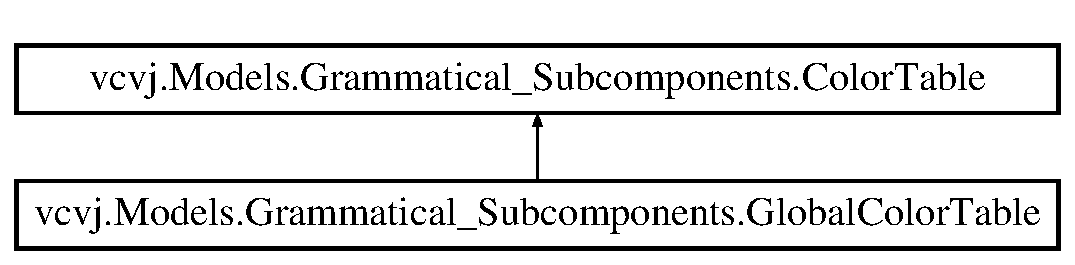
\includegraphics[height=2.000000cm]{classvcvj_1_1_models_1_1_grammatical___subcomponents_1_1_global_color_table}
\end{center}
\end{figure}
\subsection*{Additional Inherited Members}


\subsection{Detailed Description}
A block containing global information about colors used. 



The documentation for this class was generated from the following file\+:\begin{DoxyCompactItemize}
\item 
vcvj/\+Models/\+Grammatical Subcomponents/Color\+Tables.\+cs\end{DoxyCompactItemize}

\hypertarget{classvcvj_1_1_models_1_1_grammatical___components_1_1_graphic_block}{}\section{vcvj.\+Models.\+Grammatical\+\_\+\+Components.\+Graphic\+Block Class Reference}
\label{classvcvj_1_1_models_1_1_grammatical___components_1_1_graphic_block}\index{vcvj.\+Models.\+Grammatical\+\_\+\+Components.\+Graphic\+Block@{vcvj.\+Models.\+Grammatical\+\_\+\+Components.\+Graphic\+Block}}


A block containing a graphic-\/rendering block and an optional graphic control extension.  


Inheritance diagram for vcvj.\+Models.\+Grammatical\+\_\+\+Components.\+Graphic\+Block\+:\begin{figure}[H]
\begin{center}
\leavevmode
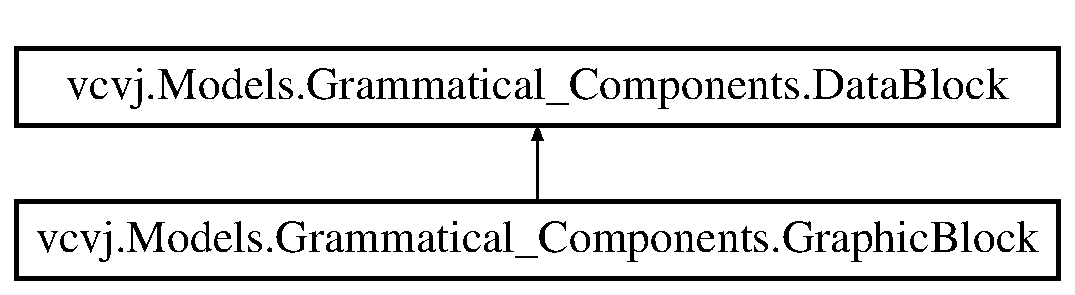
\includegraphics[height=2.000000cm]{classvcvj_1_1_models_1_1_grammatical___components_1_1_graphic_block}
\end{center}
\end{figure}
\subsection*{Properties}
\begin{DoxyCompactItemize}
\item 
\hyperlink{classvcvj_1_1_models_1_1_grammatical___subcomponents_1_1_graphic_control_extension}{Graphic\+Control\+Extension} {\bfseries Graphic\+Control\+Extension}\hspace{0.3cm}{\ttfamily  \mbox{[}get, set\mbox{]}}\hypertarget{classvcvj_1_1_models_1_1_grammatical___components_1_1_graphic_block_a4f44785d1058e29dbf194a23ea2ffff2}{}\label{classvcvj_1_1_models_1_1_grammatical___components_1_1_graphic_block_a4f44785d1058e29dbf194a23ea2ffff2}

\item 
\hyperlink{classvcvj_1_1_models_1_1_grammatical___components_1_1_graphic_rendering_block}{Graphic\+Rendering\+Block} {\bfseries Graphic\+Rendering\+Block}\hspace{0.3cm}{\ttfamily  \mbox{[}get, set\mbox{]}}\hypertarget{classvcvj_1_1_models_1_1_grammatical___components_1_1_graphic_block_a3b94cc4f51720b0cd37ecb87e8c844e4}{}\label{classvcvj_1_1_models_1_1_grammatical___components_1_1_graphic_block_a3b94cc4f51720b0cd37ecb87e8c844e4}

\end{DoxyCompactItemize}
\subsection*{Additional Inherited Members}


\subsection{Detailed Description}
A block containing a graphic-\/rendering block and an optional graphic control extension. 



The documentation for this class was generated from the following file\+:\begin{DoxyCompactItemize}
\item 
vcvj/\+Models/\+Grammatical Components/Graphic\+Block.\+cs\end{DoxyCompactItemize}

\hypertarget{classvcvj_1_1_models_1_1_grammatical___subcomponents_1_1_graphic_control_extension}{}\section{vcvj.\+Models.\+Grammatical\+\_\+\+Subcomponents.\+Graphic\+Control\+Extension Class Reference}
\label{classvcvj_1_1_models_1_1_grammatical___subcomponents_1_1_graphic_control_extension}\index{vcvj.\+Models.\+Grammatical\+\_\+\+Subcomponents.\+Graphic\+Control\+Extension@{vcvj.\+Models.\+Grammatical\+\_\+\+Subcomponents.\+Graphic\+Control\+Extension}}


An optional extension used to specify transparency settings and control animations.  


\subsection*{Public Attributes}
\begin{DoxyCompactItemize}
\item 
const int {\bfseries Total\+Block\+Length} = 8\hypertarget{classvcvj_1_1_models_1_1_grammatical___subcomponents_1_1_graphic_control_extension_a37b1009039c425e1153e67b7150d8072}{}\label{classvcvj_1_1_models_1_1_grammatical___subcomponents_1_1_graphic_control_extension_a37b1009039c425e1153e67b7150d8072}

\item 
byte\mbox{[}$\,$\mbox{]} {\bfseries Bytes} = new byte\mbox{[}Total\+Block\+Length\mbox{]}\hypertarget{classvcvj_1_1_models_1_1_grammatical___subcomponents_1_1_graphic_control_extension_a62037e4aa2974b83de3d3981af827ccc}{}\label{classvcvj_1_1_models_1_1_grammatical___subcomponents_1_1_graphic_control_extension_a62037e4aa2974b83de3d3981af827ccc}

\end{DoxyCompactItemize}
\subsection*{Properties}
\begin{DoxyCompactItemize}
\item 
int {\bfseries Block\+Size}\hspace{0.3cm}{\ttfamily  \mbox{[}get, set\mbox{]}}\hypertarget{classvcvj_1_1_models_1_1_grammatical___subcomponents_1_1_graphic_control_extension_a5aa3b81589ed47175bdf2f9cec6aa8e7}{}\label{classvcvj_1_1_models_1_1_grammatical___subcomponents_1_1_graphic_control_extension_a5aa3b81589ed47175bdf2f9cec6aa8e7}

\item 
string {\bfseries Packed\+Field}\hspace{0.3cm}{\ttfamily  \mbox{[}get, set\mbox{]}}\hypertarget{classvcvj_1_1_models_1_1_grammatical___subcomponents_1_1_graphic_control_extension_a28a2fde511ee8c68a9a1259e4004c7f8}{}\label{classvcvj_1_1_models_1_1_grammatical___subcomponents_1_1_graphic_control_extension_a28a2fde511ee8c68a9a1259e4004c7f8}

\item 
int {\bfseries Disposal\+Method}\hspace{0.3cm}{\ttfamily  \mbox{[}get, set\mbox{]}}\hypertarget{classvcvj_1_1_models_1_1_grammatical___subcomponents_1_1_graphic_control_extension_a9ecfcb6a0c4a1cd3095ffc74937b8aae}{}\label{classvcvj_1_1_models_1_1_grammatical___subcomponents_1_1_graphic_control_extension_a9ecfcb6a0c4a1cd3095ffc74937b8aae}

\item 
bool {\bfseries User\+Input\+Flag}\hspace{0.3cm}{\ttfamily  \mbox{[}get, set\mbox{]}}\hypertarget{classvcvj_1_1_models_1_1_grammatical___subcomponents_1_1_graphic_control_extension_a1f6e112d4c4a2d57e1c1dfd59ec61922}{}\label{classvcvj_1_1_models_1_1_grammatical___subcomponents_1_1_graphic_control_extension_a1f6e112d4c4a2d57e1c1dfd59ec61922}

\item 
bool {\bfseries Transparent\+Color\+Flag}\hspace{0.3cm}{\ttfamily  \mbox{[}get, set\mbox{]}}\hypertarget{classvcvj_1_1_models_1_1_grammatical___subcomponents_1_1_graphic_control_extension_ac5b58a8edbc51ef9efc77bbf86d760df}{}\label{classvcvj_1_1_models_1_1_grammatical___subcomponents_1_1_graphic_control_extension_ac5b58a8edbc51ef9efc77bbf86d760df}

\item 
int {\bfseries Delay\+Time}\hspace{0.3cm}{\ttfamily  \mbox{[}get, set\mbox{]}}\hypertarget{classvcvj_1_1_models_1_1_grammatical___subcomponents_1_1_graphic_control_extension_a2f5305024d724e80b08aa565a6cf4ea6}{}\label{classvcvj_1_1_models_1_1_grammatical___subcomponents_1_1_graphic_control_extension_a2f5305024d724e80b08aa565a6cf4ea6}

\item 
int {\bfseries Transparent\+Color\+Index}\hspace{0.3cm}{\ttfamily  \mbox{[}get, set\mbox{]}}\hypertarget{classvcvj_1_1_models_1_1_grammatical___subcomponents_1_1_graphic_control_extension_a5549c0c65d27e93cc9db2acb2b457f52}{}\label{classvcvj_1_1_models_1_1_grammatical___subcomponents_1_1_graphic_control_extension_a5549c0c65d27e93cc9db2acb2b457f52}

\end{DoxyCompactItemize}


\subsection{Detailed Description}
An optional extension used to specify transparency settings and control animations. 



The documentation for this class was generated from the following file\+:\begin{DoxyCompactItemize}
\item 
vcvj/\+Models/\+Grammatical Subcomponents/Graphic\+Control\+Extension.\+cs\end{DoxyCompactItemize}

\hypertarget{classvcvj_1_1_models_1_1_grammatical___components_1_1_graphic_rendering_block}{}\section{vcvj.\+Models.\+Grammatical\+\_\+\+Components.\+Graphic\+Rendering\+Block Class Reference}
\label{classvcvj_1_1_models_1_1_grammatical___components_1_1_graphic_rendering_block}\index{vcvj.\+Models.\+Grammatical\+\_\+\+Components.\+Graphic\+Rendering\+Block@{vcvj.\+Models.\+Grammatical\+\_\+\+Components.\+Graphic\+Rendering\+Block}}


Represents table-\/based images or plain text extensions.  


Inheritance diagram for vcvj.\+Models.\+Grammatical\+\_\+\+Components.\+Graphic\+Rendering\+Block\+:\begin{figure}[H]
\begin{center}
\leavevmode
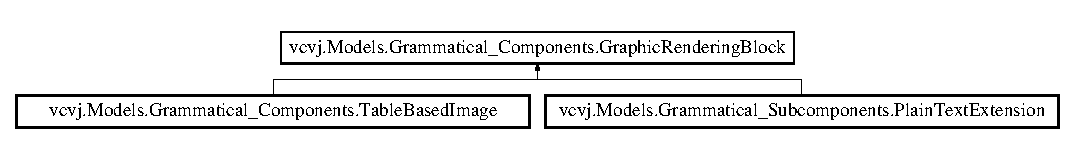
\includegraphics[height=1.489362cm]{classvcvj_1_1_models_1_1_grammatical___components_1_1_graphic_rendering_block}
\end{center}
\end{figure}
\subsection*{Public Member Functions}
\begin{DoxyCompactItemize}
\item 
\hyperlink{classvcvj_1_1_models_1_1_grammatical___components_1_1_table_based_image}{Table\+Based\+Image} \hyperlink{classvcvj_1_1_models_1_1_grammatical___components_1_1_graphic_rendering_block_a0373c25b75cc4d867d3e0cf3155046c8}{To\+Table\+Based\+Image} ()
\begin{DoxyCompactList}\small\item\em Casts the \hyperlink{classvcvj_1_1_models_1_1_grammatical___components_1_1_graphic_rendering_block}{Graphic\+Rendering\+Block} into a \hyperlink{classvcvj_1_1_models_1_1_grammatical___components_1_1_table_based_image}{Table\+Based\+Image}. \end{DoxyCompactList}\item 
\hyperlink{classvcvj_1_1_models_1_1_grammatical___subcomponents_1_1_plain_text_extension}{Plain\+Text\+Extension} \hyperlink{classvcvj_1_1_models_1_1_grammatical___components_1_1_graphic_rendering_block_aeb72aff7c9a375cf9c63f7465596dea6}{To\+Plain\+Text\+Extension} ()
\begin{DoxyCompactList}\small\item\em Casts the \hyperlink{classvcvj_1_1_models_1_1_grammatical___components_1_1_graphic_rendering_block}{Graphic\+Rendering\+Block} into a Plain\+Text\+Extension. \end{DoxyCompactList}\end{DoxyCompactItemize}
\subsection*{Properties}
\begin{DoxyCompactItemize}
\item 
bool \hyperlink{classvcvj_1_1_models_1_1_grammatical___components_1_1_graphic_rendering_block_a66ec3f983a1b11b333449336afe4e1e0}{Is\+Table\+Based\+Image}\hspace{0.3cm}{\ttfamily  \mbox{[}get\mbox{]}}
\begin{DoxyCompactList}\small\item\em Determines whether or not a \hyperlink{classvcvj_1_1_models_1_1_grammatical___components_1_1_graphic_rendering_block}{Graphic\+Rendering\+Block} represents a \hyperlink{classvcvj_1_1_models_1_1_grammatical___components_1_1_table_based_image}{Table\+Based\+Image}. \end{DoxyCompactList}\item 
bool \hyperlink{classvcvj_1_1_models_1_1_grammatical___components_1_1_graphic_rendering_block_ad59385e1e9d5ac39a87211436ff0304a}{Is\+Plain\+Text\+Extension}\hspace{0.3cm}{\ttfamily  \mbox{[}get\mbox{]}}
\begin{DoxyCompactList}\small\item\em Determines whether or not a \hyperlink{classvcvj_1_1_models_1_1_grammatical___components_1_1_graphic_rendering_block}{Graphic\+Rendering\+Block} represents a Plain\+Text\+Extension. \end{DoxyCompactList}\end{DoxyCompactItemize}


\subsection{Detailed Description}
Represents table-\/based images or plain text extensions. 



\subsection{Member Function Documentation}
\index{vcvj\+::\+Models\+::\+Grammatical\+\_\+\+Components\+::\+Graphic\+Rendering\+Block@{vcvj\+::\+Models\+::\+Grammatical\+\_\+\+Components\+::\+Graphic\+Rendering\+Block}!To\+Plain\+Text\+Extension@{To\+Plain\+Text\+Extension}}
\index{To\+Plain\+Text\+Extension@{To\+Plain\+Text\+Extension}!vcvj\+::\+Models\+::\+Grammatical\+\_\+\+Components\+::\+Graphic\+Rendering\+Block@{vcvj\+::\+Models\+::\+Grammatical\+\_\+\+Components\+::\+Graphic\+Rendering\+Block}}
\subsubsection[{\texorpdfstring{To\+Plain\+Text\+Extension()}{ToPlainTextExtension()}}]{\setlength{\rightskip}{0pt plus 5cm}{\bf Plain\+Text\+Extension} vcvj.\+Models.\+Grammatical\+\_\+\+Components.\+Graphic\+Rendering\+Block.\+To\+Plain\+Text\+Extension (
\begin{DoxyParamCaption}
{}
\end{DoxyParamCaption}
)\hspace{0.3cm}{\ttfamily [inline]}}\hypertarget{classvcvj_1_1_models_1_1_grammatical___components_1_1_graphic_rendering_block_aeb72aff7c9a375cf9c63f7465596dea6}{}\label{classvcvj_1_1_models_1_1_grammatical___components_1_1_graphic_rendering_block_aeb72aff7c9a375cf9c63f7465596dea6}


Casts the \hyperlink{classvcvj_1_1_models_1_1_grammatical___components_1_1_graphic_rendering_block}{Graphic\+Rendering\+Block} into a Plain\+Text\+Extension. 

\index{vcvj\+::\+Models\+::\+Grammatical\+\_\+\+Components\+::\+Graphic\+Rendering\+Block@{vcvj\+::\+Models\+::\+Grammatical\+\_\+\+Components\+::\+Graphic\+Rendering\+Block}!To\+Table\+Based\+Image@{To\+Table\+Based\+Image}}
\index{To\+Table\+Based\+Image@{To\+Table\+Based\+Image}!vcvj\+::\+Models\+::\+Grammatical\+\_\+\+Components\+::\+Graphic\+Rendering\+Block@{vcvj\+::\+Models\+::\+Grammatical\+\_\+\+Components\+::\+Graphic\+Rendering\+Block}}
\subsubsection[{\texorpdfstring{To\+Table\+Based\+Image()}{ToTableBasedImage()}}]{\setlength{\rightskip}{0pt plus 5cm}{\bf Table\+Based\+Image} vcvj.\+Models.\+Grammatical\+\_\+\+Components.\+Graphic\+Rendering\+Block.\+To\+Table\+Based\+Image (
\begin{DoxyParamCaption}
{}
\end{DoxyParamCaption}
)\hspace{0.3cm}{\ttfamily [inline]}}\hypertarget{classvcvj_1_1_models_1_1_grammatical___components_1_1_graphic_rendering_block_a0373c25b75cc4d867d3e0cf3155046c8}{}\label{classvcvj_1_1_models_1_1_grammatical___components_1_1_graphic_rendering_block_a0373c25b75cc4d867d3e0cf3155046c8}


Casts the \hyperlink{classvcvj_1_1_models_1_1_grammatical___components_1_1_graphic_rendering_block}{Graphic\+Rendering\+Block} into a \hyperlink{classvcvj_1_1_models_1_1_grammatical___components_1_1_table_based_image}{Table\+Based\+Image}. 



\subsection{Property Documentation}
\index{vcvj\+::\+Models\+::\+Grammatical\+\_\+\+Components\+::\+Graphic\+Rendering\+Block@{vcvj\+::\+Models\+::\+Grammatical\+\_\+\+Components\+::\+Graphic\+Rendering\+Block}!Is\+Plain\+Text\+Extension@{Is\+Plain\+Text\+Extension}}
\index{Is\+Plain\+Text\+Extension@{Is\+Plain\+Text\+Extension}!vcvj\+::\+Models\+::\+Grammatical\+\_\+\+Components\+::\+Graphic\+Rendering\+Block@{vcvj\+::\+Models\+::\+Grammatical\+\_\+\+Components\+::\+Graphic\+Rendering\+Block}}
\subsubsection[{\texorpdfstring{Is\+Plain\+Text\+Extension}{IsPlainTextExtension}}]{\setlength{\rightskip}{0pt plus 5cm}bool vcvj.\+Models.\+Grammatical\+\_\+\+Components.\+Graphic\+Rendering\+Block.\+Is\+Plain\+Text\+Extension\hspace{0.3cm}{\ttfamily [get]}}\hypertarget{classvcvj_1_1_models_1_1_grammatical___components_1_1_graphic_rendering_block_ad59385e1e9d5ac39a87211436ff0304a}{}\label{classvcvj_1_1_models_1_1_grammatical___components_1_1_graphic_rendering_block_ad59385e1e9d5ac39a87211436ff0304a}


Determines whether or not a \hyperlink{classvcvj_1_1_models_1_1_grammatical___components_1_1_graphic_rendering_block}{Graphic\+Rendering\+Block} represents a Plain\+Text\+Extension. 

\index{vcvj\+::\+Models\+::\+Grammatical\+\_\+\+Components\+::\+Graphic\+Rendering\+Block@{vcvj\+::\+Models\+::\+Grammatical\+\_\+\+Components\+::\+Graphic\+Rendering\+Block}!Is\+Table\+Based\+Image@{Is\+Table\+Based\+Image}}
\index{Is\+Table\+Based\+Image@{Is\+Table\+Based\+Image}!vcvj\+::\+Models\+::\+Grammatical\+\_\+\+Components\+::\+Graphic\+Rendering\+Block@{vcvj\+::\+Models\+::\+Grammatical\+\_\+\+Components\+::\+Graphic\+Rendering\+Block}}
\subsubsection[{\texorpdfstring{Is\+Table\+Based\+Image}{IsTableBasedImage}}]{\setlength{\rightskip}{0pt plus 5cm}bool vcvj.\+Models.\+Grammatical\+\_\+\+Components.\+Graphic\+Rendering\+Block.\+Is\+Table\+Based\+Image\hspace{0.3cm}{\ttfamily [get]}}\hypertarget{classvcvj_1_1_models_1_1_grammatical___components_1_1_graphic_rendering_block_a66ec3f983a1b11b333449336afe4e1e0}{}\label{classvcvj_1_1_models_1_1_grammatical___components_1_1_graphic_rendering_block_a66ec3f983a1b11b333449336afe4e1e0}


Determines whether or not a \hyperlink{classvcvj_1_1_models_1_1_grammatical___components_1_1_graphic_rendering_block}{Graphic\+Rendering\+Block} represents a \hyperlink{classvcvj_1_1_models_1_1_grammatical___components_1_1_table_based_image}{Table\+Based\+Image}. 



The documentation for this class was generated from the following file\+:\begin{DoxyCompactItemize}
\item 
vcvj/\+Models/\+Grammatical Components/Graphic\+Rendering\+Block.\+cs\end{DoxyCompactItemize}

\hypertarget{classvcvj_1_1_models_1_1_grammatical___subcomponents_1_1_header}{}\section{vcvj.\+Models.\+Grammatical\+\_\+\+Subcomponents.\+Header Class Reference}
\label{classvcvj_1_1_models_1_1_grammatical___subcomponents_1_1_header}\index{vcvj.\+Models.\+Grammatical\+\_\+\+Subcomponents.\+Header@{vcvj.\+Models.\+Grammatical\+\_\+\+Subcomponents.\+Header}}


The block which contains the image\textquotesingle{}s signature and version encoding.  


\subsection*{Public Attributes}
\begin{DoxyCompactItemize}
\item 
const int {\bfseries Total\+Block\+Length} = 6\hypertarget{classvcvj_1_1_models_1_1_grammatical___subcomponents_1_1_header_a4c41af980a2ee54f9d435dce794bbc23}{}\label{classvcvj_1_1_models_1_1_grammatical___subcomponents_1_1_header_a4c41af980a2ee54f9d435dce794bbc23}

\item 
byte\mbox{[}$\,$\mbox{]} {\bfseries Bytes} = new byte\mbox{[}Header.\+Total\+Block\+Length\mbox{]}\hypertarget{classvcvj_1_1_models_1_1_grammatical___subcomponents_1_1_header_a16d44e9018738a6b01d61a46015059be}{}\label{classvcvj_1_1_models_1_1_grammatical___subcomponents_1_1_header_a16d44e9018738a6b01d61a46015059be}

\end{DoxyCompactItemize}


\subsection{Detailed Description}
The block which contains the image\textquotesingle{}s signature and version encoding. 



The documentation for this class was generated from the following file\+:\begin{DoxyCompactItemize}
\item 
vcvj/\+Models/\+Grammatical Subcomponents/Header.\+cs\end{DoxyCompactItemize}

\hypertarget{classvcvj_1_1_models_1_1_grammatical___subcomponents_1_1_image_data}{}\section{vcvj.\+Models.\+Grammatical\+\_\+\+Subcomponents.\+Image\+Data Class Reference}
\label{classvcvj_1_1_models_1_1_grammatical___subcomponents_1_1_image_data}\index{vcvj.\+Models.\+Grammatical\+\_\+\+Subcomponents.\+Image\+Data@{vcvj.\+Models.\+Grammatical\+\_\+\+Subcomponents.\+Image\+Data}}
\subsection*{Public Member Functions}
\begin{DoxyCompactItemize}
\item 
\hyperlink{classvcvj_1_1_models_1_1_grammatical___subcomponents_1_1_image_data}{Image\+Data} \hyperlink{classvcvj_1_1_models_1_1_grammatical___subcomponents_1_1_image_data_ac0cbc65689a126364a6863199815e0b7}{Threshold} (byte r, byte g, byte b)
\begin{DoxyCompactList}\small\item\em Turns pixels white or black depending on whether or not their byte values exceed a given threshold. \end{DoxyCompactList}\end{DoxyCompactItemize}
\subsection*{Properties}
\begin{DoxyCompactItemize}
\item 
byte\mbox{[}$\,$\mbox{]} {\bfseries Bytes}\hspace{0.3cm}{\ttfamily  \mbox{[}get, set\mbox{]}}\hypertarget{classvcvj_1_1_models_1_1_grammatical___subcomponents_1_1_image_data_a4fb8b1e7192b92938932d3d559b1f1c0}{}\label{classvcvj_1_1_models_1_1_grammatical___subcomponents_1_1_image_data_a4fb8b1e7192b92938932d3d559b1f1c0}

\item 
int {\bfseries Total\+Block\+Length}\hspace{0.3cm}{\ttfamily  \mbox{[}get, set\mbox{]}}\hypertarget{classvcvj_1_1_models_1_1_grammatical___subcomponents_1_1_image_data_a8ad2052c4d8947c68940e464d2eb983e}{}\label{classvcvj_1_1_models_1_1_grammatical___subcomponents_1_1_image_data_a8ad2052c4d8947c68940e464d2eb983e}

\item 
int {\bfseries Lzw\+Minimum\+Code\+Size}\hspace{0.3cm}{\ttfamily  \mbox{[}get, set\mbox{]}}\hypertarget{classvcvj_1_1_models_1_1_grammatical___subcomponents_1_1_image_data_ac7920f89c775125b4a0ed4aa4f9f8366}{}\label{classvcvj_1_1_models_1_1_grammatical___subcomponents_1_1_image_data_ac7920f89c775125b4a0ed4aa4f9f8366}

\end{DoxyCompactItemize}


\subsection{Member Function Documentation}
\index{vcvj\+::\+Models\+::\+Grammatical\+\_\+\+Subcomponents\+::\+Image\+Data@{vcvj\+::\+Models\+::\+Grammatical\+\_\+\+Subcomponents\+::\+Image\+Data}!Threshold@{Threshold}}
\index{Threshold@{Threshold}!vcvj\+::\+Models\+::\+Grammatical\+\_\+\+Subcomponents\+::\+Image\+Data@{vcvj\+::\+Models\+::\+Grammatical\+\_\+\+Subcomponents\+::\+Image\+Data}}
\subsubsection[{\texorpdfstring{Threshold(byte r, byte g, byte b)}{Threshold(byte r, byte g, byte b)}}]{\setlength{\rightskip}{0pt plus 5cm}{\bf Image\+Data} vcvj.\+Models.\+Grammatical\+\_\+\+Subcomponents.\+Image\+Data.\+Threshold (
\begin{DoxyParamCaption}
\item[{byte}]{r, }
\item[{byte}]{g, }
\item[{byte}]{b}
\end{DoxyParamCaption}
)\hspace{0.3cm}{\ttfamily [inline]}}\hypertarget{classvcvj_1_1_models_1_1_grammatical___subcomponents_1_1_image_data_ac0cbc65689a126364a6863199815e0b7}{}\label{classvcvj_1_1_models_1_1_grammatical___subcomponents_1_1_image_data_ac0cbc65689a126364a6863199815e0b7}


Turns pixels white or black depending on whether or not their byte values exceed a given threshold. 


\begin{DoxyParams}{Parameters}
{\em r} & \\
\hline
{\em g} & \\
\hline
{\em b} & \\
\hline
\end{DoxyParams}
\begin{DoxyReturn}{Returns}

\end{DoxyReturn}


The documentation for this class was generated from the following file\+:\begin{DoxyCompactItemize}
\item 
vcvj/\+Models/\+Grammatical Subcomponents/Image\+Data.\+cs\end{DoxyCompactItemize}

\hypertarget{classvcvj_1_1_models_1_1_grammatical___subcomponents_1_1_image_descriptor}{}\section{vcvj.\+Models.\+Grammatical\+\_\+\+Subcomponents.\+Image\+Descriptor Class Reference}
\label{classvcvj_1_1_models_1_1_grammatical___subcomponents_1_1_image_descriptor}\index{vcvj.\+Models.\+Grammatical\+\_\+\+Subcomponents.\+Image\+Descriptor@{vcvj.\+Models.\+Grammatical\+\_\+\+Subcomponents.\+Image\+Descriptor}}
\subsection*{Public Attributes}
\begin{DoxyCompactItemize}
\item 
byte\mbox{[}$\,$\mbox{]} {\bfseries Bytes} = new byte\mbox{[}10\mbox{]}\hypertarget{classvcvj_1_1_models_1_1_grammatical___subcomponents_1_1_image_descriptor_a72aee5acd4f3fce5e8ac56374f5ce063}{}\label{classvcvj_1_1_models_1_1_grammatical___subcomponents_1_1_image_descriptor_a72aee5acd4f3fce5e8ac56374f5ce063}

\item 
const int {\bfseries Total\+Block\+Length} = 10\hypertarget{classvcvj_1_1_models_1_1_grammatical___subcomponents_1_1_image_descriptor_a44c2202e96aba57941bb233ef3e155e9}{}\label{classvcvj_1_1_models_1_1_grammatical___subcomponents_1_1_image_descriptor_a44c2202e96aba57941bb233ef3e155e9}

\end{DoxyCompactItemize}
\subsection*{Properties}
\begin{DoxyCompactItemize}
\item 
int {\bfseries Image\+Left}\hspace{0.3cm}{\ttfamily  \mbox{[}get, set\mbox{]}}\hypertarget{classvcvj_1_1_models_1_1_grammatical___subcomponents_1_1_image_descriptor_a0960157cfa44eea760f33375df3b9b66}{}\label{classvcvj_1_1_models_1_1_grammatical___subcomponents_1_1_image_descriptor_a0960157cfa44eea760f33375df3b9b66}

\item 
int {\bfseries Image\+Top}\hspace{0.3cm}{\ttfamily  \mbox{[}get, set\mbox{]}}\hypertarget{classvcvj_1_1_models_1_1_grammatical___subcomponents_1_1_image_descriptor_a98771c28203eeaf97c3eaa9696e8f8f0}{}\label{classvcvj_1_1_models_1_1_grammatical___subcomponents_1_1_image_descriptor_a98771c28203eeaf97c3eaa9696e8f8f0}

\item 
int {\bfseries Image\+Width}\hspace{0.3cm}{\ttfamily  \mbox{[}get, set\mbox{]}}\hypertarget{classvcvj_1_1_models_1_1_grammatical___subcomponents_1_1_image_descriptor_a6cd1bba3bc8c9b1177fb0ea35d6654f0}{}\label{classvcvj_1_1_models_1_1_grammatical___subcomponents_1_1_image_descriptor_a6cd1bba3bc8c9b1177fb0ea35d6654f0}

\item 
int {\bfseries Image\+Height}\hspace{0.3cm}{\ttfamily  \mbox{[}get, set\mbox{]}}\hypertarget{classvcvj_1_1_models_1_1_grammatical___subcomponents_1_1_image_descriptor_a347930ed1105cebcfa7b6047ad6c77ea}{}\label{classvcvj_1_1_models_1_1_grammatical___subcomponents_1_1_image_descriptor_a347930ed1105cebcfa7b6047ad6c77ea}

\item 
string {\bfseries Packed\+Field}\hspace{0.3cm}{\ttfamily  \mbox{[}get, set\mbox{]}}\hypertarget{classvcvj_1_1_models_1_1_grammatical___subcomponents_1_1_image_descriptor_af61b06a4c99c8ac36b4ce5038291274a}{}\label{classvcvj_1_1_models_1_1_grammatical___subcomponents_1_1_image_descriptor_af61b06a4c99c8ac36b4ce5038291274a}

\item 
bool {\bfseries Local\+Color\+Table\+Flag}\hspace{0.3cm}{\ttfamily  \mbox{[}get, set\mbox{]}}\hypertarget{classvcvj_1_1_models_1_1_grammatical___subcomponents_1_1_image_descriptor_a33808a8ea2b3e59b3d0d7ae325c52f7f}{}\label{classvcvj_1_1_models_1_1_grammatical___subcomponents_1_1_image_descriptor_a33808a8ea2b3e59b3d0d7ae325c52f7f}

\item 
bool {\bfseries Interlace\+Flag}\hspace{0.3cm}{\ttfamily  \mbox{[}get, set\mbox{]}}\hypertarget{classvcvj_1_1_models_1_1_grammatical___subcomponents_1_1_image_descriptor_a0ae70da55f68a691b4a4813dd3bb5032}{}\label{classvcvj_1_1_models_1_1_grammatical___subcomponents_1_1_image_descriptor_a0ae70da55f68a691b4a4813dd3bb5032}

\item 
bool {\bfseries Sort\+Flag}\hspace{0.3cm}{\ttfamily  \mbox{[}get, set\mbox{]}}\hypertarget{classvcvj_1_1_models_1_1_grammatical___subcomponents_1_1_image_descriptor_aef8028c8256023b093f28d47f6b64b2a}{}\label{classvcvj_1_1_models_1_1_grammatical___subcomponents_1_1_image_descriptor_aef8028c8256023b093f28d47f6b64b2a}

\item 
int {\bfseries Reserved\+For\+Future\+Use}\hspace{0.3cm}{\ttfamily  \mbox{[}get, set\mbox{]}}\hypertarget{classvcvj_1_1_models_1_1_grammatical___subcomponents_1_1_image_descriptor_a54f2233309eecfffda5779e8f419536a}{}\label{classvcvj_1_1_models_1_1_grammatical___subcomponents_1_1_image_descriptor_a54f2233309eecfffda5779e8f419536a}

\item 
int {\bfseries Local\+Color\+Table\+Length}\hspace{0.3cm}{\ttfamily  \mbox{[}get, set\mbox{]}}\hypertarget{classvcvj_1_1_models_1_1_grammatical___subcomponents_1_1_image_descriptor_ae3636ab9082c33e5d04cfa33c85be44c}{}\label{classvcvj_1_1_models_1_1_grammatical___subcomponents_1_1_image_descriptor_ae3636ab9082c33e5d04cfa33c85be44c}

\end{DoxyCompactItemize}


The documentation for this class was generated from the following file\+:\begin{DoxyCompactItemize}
\item 
vcvj/\+Models/\+Grammatical Subcomponents/Image\+Descriptor.\+cs\end{DoxyCompactItemize}

\hypertarget{classvcvj_1_1_models_1_1_grammatical___subcomponents_1_1_local_color_table}{}\section{vcvj.\+Models.\+Grammatical\+\_\+\+Subcomponents.\+Local\+Color\+Table Class Reference}
\label{classvcvj_1_1_models_1_1_grammatical___subcomponents_1_1_local_color_table}\index{vcvj.\+Models.\+Grammatical\+\_\+\+Subcomponents.\+Local\+Color\+Table@{vcvj.\+Models.\+Grammatical\+\_\+\+Subcomponents.\+Local\+Color\+Table}}


A block containing local information about colors used, relative to a specific frame.  


Inheritance diagram for vcvj.\+Models.\+Grammatical\+\_\+\+Subcomponents.\+Local\+Color\+Table\+:\begin{figure}[H]
\begin{center}
\leavevmode
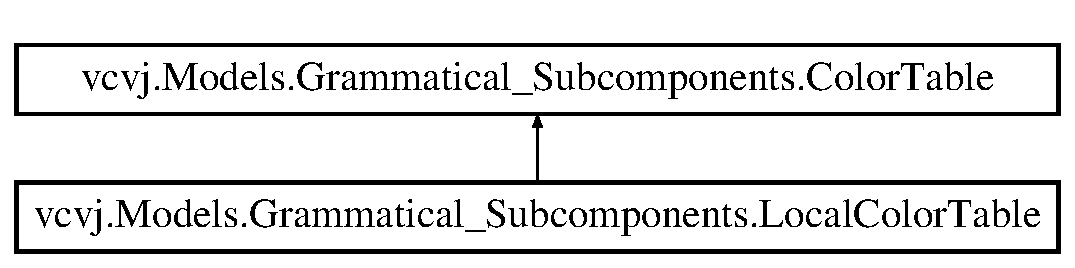
\includegraphics[height=2.000000cm]{classvcvj_1_1_models_1_1_grammatical___subcomponents_1_1_local_color_table}
\end{center}
\end{figure}
\subsection*{Additional Inherited Members}


\subsection{Detailed Description}
A block containing local information about colors used, relative to a specific frame. 



The documentation for this class was generated from the following file\+:\begin{DoxyCompactItemize}
\item 
vcvj/\+Models/\+Grammatical Subcomponents/Color\+Tables.\+cs\end{DoxyCompactItemize}

\hypertarget{classvcvj_1_1_models_1_1_grammatical___components_1_1_logical_screen}{}\section{vcvj.\+Models.\+Grammatical\+\_\+\+Components.\+Logical\+Screen Class Reference}
\label{classvcvj_1_1_models_1_1_grammatical___components_1_1_logical_screen}\index{vcvj.\+Models.\+Grammatical\+\_\+\+Components.\+Logical\+Screen@{vcvj.\+Models.\+Grammatical\+\_\+\+Components.\+Logical\+Screen}}


A block containing the logical screen descriptor and the optional global color table.  


\subsection*{Properties}
\begin{DoxyCompactItemize}
\item 
\hyperlink{classvcvj_1_1_models_1_1_grammatical___subcomponents_1_1_logical_screen_descriptor}{Logical\+Screen\+Descriptor} {\bfseries Logical\+Screen\+Descriptor}\hspace{0.3cm}{\ttfamily  \mbox{[}get, set\mbox{]}}\hypertarget{classvcvj_1_1_models_1_1_grammatical___components_1_1_logical_screen_a07dbc50b82ef62ebf583d1d8be22a466}{}\label{classvcvj_1_1_models_1_1_grammatical___components_1_1_logical_screen_a07dbc50b82ef62ebf583d1d8be22a466}

\item 
\hyperlink{classvcvj_1_1_models_1_1_grammatical___subcomponents_1_1_global_color_table}{Global\+Color\+Table} {\bfseries Global\+Color\+Table}\hspace{0.3cm}{\ttfamily  \mbox{[}get, set\mbox{]}}\hypertarget{classvcvj_1_1_models_1_1_grammatical___components_1_1_logical_screen_aa51f46460d3ed264e94ff44d0a62547b}{}\label{classvcvj_1_1_models_1_1_grammatical___components_1_1_logical_screen_aa51f46460d3ed264e94ff44d0a62547b}

\item 
int {\bfseries Total\+Block\+Length}\hspace{0.3cm}{\ttfamily  \mbox{[}get\mbox{]}}\hypertarget{classvcvj_1_1_models_1_1_grammatical___components_1_1_logical_screen_a12dd15d4faa29fbf148b70055e843373}{}\label{classvcvj_1_1_models_1_1_grammatical___components_1_1_logical_screen_a12dd15d4faa29fbf148b70055e843373}

\end{DoxyCompactItemize}


\subsection{Detailed Description}
A block containing the logical screen descriptor and the optional global color table. 



The documentation for this class was generated from the following file\+:\begin{DoxyCompactItemize}
\item 
vcvj/\+Models/\+Grammatical Components/Logical\+Screen.\+cs\end{DoxyCompactItemize}

\hypertarget{classvcvj_1_1_models_1_1_grammatical___subcomponents_1_1_logical_screen_descriptor}{}\section{vcvj.\+Models.\+Grammatical\+\_\+\+Subcomponents.\+Logical\+Screen\+Descriptor Class Reference}
\label{classvcvj_1_1_models_1_1_grammatical___subcomponents_1_1_logical_screen_descriptor}\index{vcvj.\+Models.\+Grammatical\+\_\+\+Subcomponents.\+Logical\+Screen\+Descriptor@{vcvj.\+Models.\+Grammatical\+\_\+\+Subcomponents.\+Logical\+Screen\+Descriptor}}


The block which contains data regarding the canvas dimensions, colors used, resolution, and pixel aspect ratios.  


\subsection*{Public Attributes}
\begin{DoxyCompactItemize}
\item 
const int {\bfseries Total\+Block\+Length} = 7\hypertarget{classvcvj_1_1_models_1_1_grammatical___subcomponents_1_1_logical_screen_descriptor_a99fe685a6b7979b4a587e6c39b6102a4}{}\label{classvcvj_1_1_models_1_1_grammatical___subcomponents_1_1_logical_screen_descriptor_a99fe685a6b7979b4a587e6c39b6102a4}

\item 
byte\mbox{[}$\,$\mbox{]} {\bfseries Bytes} = new byte\mbox{[}Logical\+Screen\+Descriptor.\+Total\+Block\+Length\mbox{]}\hypertarget{classvcvj_1_1_models_1_1_grammatical___subcomponents_1_1_logical_screen_descriptor_aef4aab2853527069b9711047cae22f7a}{}\label{classvcvj_1_1_models_1_1_grammatical___subcomponents_1_1_logical_screen_descriptor_aef4aab2853527069b9711047cae22f7a}

\end{DoxyCompactItemize}
\subsection*{Properties}
\begin{DoxyCompactItemize}
\item 
int {\bfseries Canvas\+Width}\hspace{0.3cm}{\ttfamily  \mbox{[}get, set\mbox{]}}\hypertarget{classvcvj_1_1_models_1_1_grammatical___subcomponents_1_1_logical_screen_descriptor_ad465d0a28fc8160c752f69293c4d4b3d}{}\label{classvcvj_1_1_models_1_1_grammatical___subcomponents_1_1_logical_screen_descriptor_ad465d0a28fc8160c752f69293c4d4b3d}

\item 
int {\bfseries Canvas\+Height}\hspace{0.3cm}{\ttfamily  \mbox{[}get, set\mbox{]}}\hypertarget{classvcvj_1_1_models_1_1_grammatical___subcomponents_1_1_logical_screen_descriptor_a0422af0f85c85e41745aca0704d1d817}{}\label{classvcvj_1_1_models_1_1_grammatical___subcomponents_1_1_logical_screen_descriptor_a0422af0f85c85e41745aca0704d1d817}

\item 
string {\bfseries Packed\+Field}\hspace{0.3cm}{\ttfamily  \mbox{[}get, set\mbox{]}}\hypertarget{classvcvj_1_1_models_1_1_grammatical___subcomponents_1_1_logical_screen_descriptor_a421a1983991a42ded654b56b7e3d90bc}{}\label{classvcvj_1_1_models_1_1_grammatical___subcomponents_1_1_logical_screen_descriptor_a421a1983991a42ded654b56b7e3d90bc}

\item 
int {\bfseries Background\+Color\+Index}\hspace{0.3cm}{\ttfamily  \mbox{[}get, set\mbox{]}}\hypertarget{classvcvj_1_1_models_1_1_grammatical___subcomponents_1_1_logical_screen_descriptor_a4e0c20c79d2605831b2d606d4487715c}{}\label{classvcvj_1_1_models_1_1_grammatical___subcomponents_1_1_logical_screen_descriptor_a4e0c20c79d2605831b2d606d4487715c}

\item 
int {\bfseries Pixel\+Aspect\+Ratio}\hspace{0.3cm}{\ttfamily  \mbox{[}get, set\mbox{]}}\hypertarget{classvcvj_1_1_models_1_1_grammatical___subcomponents_1_1_logical_screen_descriptor_a8eb65a69495467caedf2db952308e10f}{}\label{classvcvj_1_1_models_1_1_grammatical___subcomponents_1_1_logical_screen_descriptor_a8eb65a69495467caedf2db952308e10f}

\item 
int {\bfseries Color\+Resolution}\hspace{0.3cm}{\ttfamily  \mbox{[}get, set\mbox{]}}\hypertarget{classvcvj_1_1_models_1_1_grammatical___subcomponents_1_1_logical_screen_descriptor_ae23bde3db40845040209a5cf9416324e}{}\label{classvcvj_1_1_models_1_1_grammatical___subcomponents_1_1_logical_screen_descriptor_ae23bde3db40845040209a5cf9416324e}

\item 
bool {\bfseries Sort\+Flag}\hspace{0.3cm}{\ttfamily  \mbox{[}get, set\mbox{]}}\hypertarget{classvcvj_1_1_models_1_1_grammatical___subcomponents_1_1_logical_screen_descriptor_aa944c12cb8d8709e79dd1ac81e4f03da}{}\label{classvcvj_1_1_models_1_1_grammatical___subcomponents_1_1_logical_screen_descriptor_aa944c12cb8d8709e79dd1ac81e4f03da}

\item 
bool {\bfseries Has\+Global\+Color\+Table}\hspace{0.3cm}{\ttfamily  \mbox{[}get, set\mbox{]}}\hypertarget{classvcvj_1_1_models_1_1_grammatical___subcomponents_1_1_logical_screen_descriptor_a19df8fe996380b8d64909615efc420a0}{}\label{classvcvj_1_1_models_1_1_grammatical___subcomponents_1_1_logical_screen_descriptor_a19df8fe996380b8d64909615efc420a0}

\item 
int {\bfseries Global\+Color\+Table\+Size}\hspace{0.3cm}{\ttfamily  \mbox{[}get, set\mbox{]}}\hypertarget{classvcvj_1_1_models_1_1_grammatical___subcomponents_1_1_logical_screen_descriptor_a7d4bf15cab57a46e1ba586edea1cf70b}{}\label{classvcvj_1_1_models_1_1_grammatical___subcomponents_1_1_logical_screen_descriptor_a7d4bf15cab57a46e1ba586edea1cf70b}

\item 
int {\bfseries Global\+Color\+Table\+Length}\hspace{0.3cm}{\ttfamily  \mbox{[}get, set\mbox{]}}\hypertarget{classvcvj_1_1_models_1_1_grammatical___subcomponents_1_1_logical_screen_descriptor_abbb6e91992e8f02f4c9d0268b41eb5ef}{}\label{classvcvj_1_1_models_1_1_grammatical___subcomponents_1_1_logical_screen_descriptor_abbb6e91992e8f02f4c9d0268b41eb5ef}

\end{DoxyCompactItemize}


\subsection{Detailed Description}
The block which contains data regarding the canvas dimensions, colors used, resolution, and pixel aspect ratios. 



The documentation for this class was generated from the following file\+:\begin{DoxyCompactItemize}
\item 
vcvj/\+Models/\+Grammatical Subcomponents/Logical\+Screen\+Descriptor.\+cs\end{DoxyCompactItemize}

\hypertarget{classvcvj_1_1_models_1_1_grammatical___subcomponents_1_1_plain_text_extension}{}\section{vcvj.\+Models.\+Grammatical\+\_\+\+Subcomponents.\+Plain\+Text\+Extension Class Reference}
\label{classvcvj_1_1_models_1_1_grammatical___subcomponents_1_1_plain_text_extension}\index{vcvj.\+Models.\+Grammatical\+\_\+\+Subcomponents.\+Plain\+Text\+Extension@{vcvj.\+Models.\+Grammatical\+\_\+\+Subcomponents.\+Plain\+Text\+Extension}}


An extension containing captions.  


Inheritance diagram for vcvj.\+Models.\+Grammatical\+\_\+\+Subcomponents.\+Plain\+Text\+Extension\+:\begin{figure}[H]
\begin{center}
\leavevmode
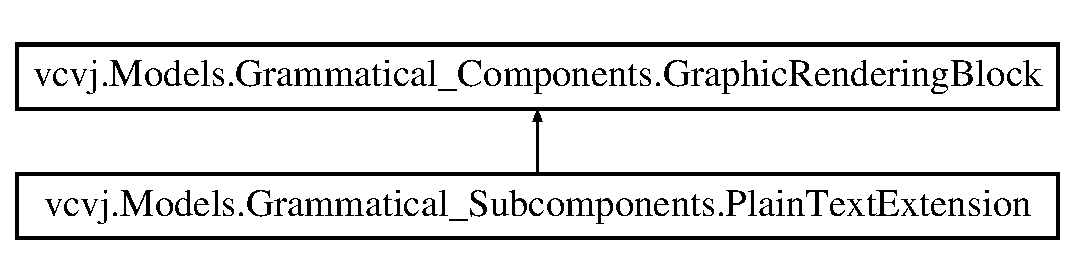
\includegraphics[height=2.000000cm]{classvcvj_1_1_models_1_1_grammatical___subcomponents_1_1_plain_text_extension}
\end{center}
\end{figure}
\subsection*{Public Member Functions}
\begin{DoxyCompactItemize}
\item 
\hyperlink{classvcvj_1_1_models_1_1_grammatical___subcomponents_1_1_plain_text_extension_a9c11305040871f3d087375996b158e50}{Plain\+Text\+Extension} (byte\mbox{[}$\,$\mbox{]} bytes)
\begin{DoxyCompactList}\small\item\em Populates the Plain Text Extension byte\mbox{[}\mbox{]} from the source image, and performs lexical parsing on the array. \end{DoxyCompactList}\end{DoxyCompactItemize}
\subsection*{Properties}
\begin{DoxyCompactItemize}
\item 
byte\mbox{[}$\,$\mbox{]} {\bfseries Bytes}\hspace{0.3cm}{\ttfamily  \mbox{[}get, set\mbox{]}}\hypertarget{classvcvj_1_1_models_1_1_grammatical___subcomponents_1_1_plain_text_extension_a2231e7d8faeb082581fceaa43db622b5}{}\label{classvcvj_1_1_models_1_1_grammatical___subcomponents_1_1_plain_text_extension_a2231e7d8faeb082581fceaa43db622b5}

\item 
int {\bfseries Total\+Block\+Length}\hspace{0.3cm}{\ttfamily  \mbox{[}get, set\mbox{]}}\hypertarget{classvcvj_1_1_models_1_1_grammatical___subcomponents_1_1_plain_text_extension_aa45cd181ae9b43c515cacef9d5be8230}{}\label{classvcvj_1_1_models_1_1_grammatical___subcomponents_1_1_plain_text_extension_aa45cd181ae9b43c515cacef9d5be8230}

\item 
int {\bfseries Block\+Size}\hspace{0.3cm}{\ttfamily  \mbox{[}get, set\mbox{]}}\hypertarget{classvcvj_1_1_models_1_1_grammatical___subcomponents_1_1_plain_text_extension_a3a11ca8960b44f3d1bde3071c8e843c8}{}\label{classvcvj_1_1_models_1_1_grammatical___subcomponents_1_1_plain_text_extension_a3a11ca8960b44f3d1bde3071c8e843c8}

\item 
string {\bfseries Caption}\hspace{0.3cm}{\ttfamily  \mbox{[}get, set\mbox{]}}\hypertarget{classvcvj_1_1_models_1_1_grammatical___subcomponents_1_1_plain_text_extension_ab9ac764c21121652f0508daa503c0786}{}\label{classvcvj_1_1_models_1_1_grammatical___subcomponents_1_1_plain_text_extension_ab9ac764c21121652f0508daa503c0786}

\end{DoxyCompactItemize}


\subsection{Detailed Description}
An extension containing captions. 



\subsection{Constructor \& Destructor Documentation}
\index{vcvj\+::\+Models\+::\+Grammatical\+\_\+\+Subcomponents\+::\+Plain\+Text\+Extension@{vcvj\+::\+Models\+::\+Grammatical\+\_\+\+Subcomponents\+::\+Plain\+Text\+Extension}!Plain\+Text\+Extension@{Plain\+Text\+Extension}}
\index{Plain\+Text\+Extension@{Plain\+Text\+Extension}!vcvj\+::\+Models\+::\+Grammatical\+\_\+\+Subcomponents\+::\+Plain\+Text\+Extension@{vcvj\+::\+Models\+::\+Grammatical\+\_\+\+Subcomponents\+::\+Plain\+Text\+Extension}}
\subsubsection[{\texorpdfstring{Plain\+Text\+Extension(byte[] bytes)}{PlainTextExtension(byte[] bytes)}}]{\setlength{\rightskip}{0pt plus 5cm}vcvj.\+Models.\+Grammatical\+\_\+\+Subcomponents.\+Plain\+Text\+Extension.\+Plain\+Text\+Extension (
\begin{DoxyParamCaption}
\item[{byte\mbox{[}$\,$\mbox{]}}]{bytes}
\end{DoxyParamCaption}
)\hspace{0.3cm}{\ttfamily [inline]}}\hypertarget{classvcvj_1_1_models_1_1_grammatical___subcomponents_1_1_plain_text_extension_a9c11305040871f3d087375996b158e50}{}\label{classvcvj_1_1_models_1_1_grammatical___subcomponents_1_1_plain_text_extension_a9c11305040871f3d087375996b158e50}


Populates the Plain Text Extension byte\mbox{[}\mbox{]} from the source image, and performs lexical parsing on the array. 


\begin{DoxyParams}{Parameters}
{\em bytes} & \\
\hline
\end{DoxyParams}


The documentation for this class was generated from the following file\+:\begin{DoxyCompactItemize}
\item 
vcvj/\+Models/\+Grammatical Subcomponents/Plain\+Text\+Extension.\+cs\end{DoxyCompactItemize}

\hypertarget{classvcvj_1_1_models_1_1_grammatical___components_1_1_special_purpose_block}{}\section{vcvj.\+Models.\+Grammatical\+\_\+\+Components.\+Special\+Purpose\+Block Class Reference}
\label{classvcvj_1_1_models_1_1_grammatical___components_1_1_special_purpose_block}\index{vcvj.\+Models.\+Grammatical\+\_\+\+Components.\+Special\+Purpose\+Block@{vcvj.\+Models.\+Grammatical\+\_\+\+Components.\+Special\+Purpose\+Block}}


Represents either an application extension or a comment extension.  


Inheritance diagram for vcvj.\+Models.\+Grammatical\+\_\+\+Components.\+Special\+Purpose\+Block\+:\begin{figure}[H]
\begin{center}
\leavevmode
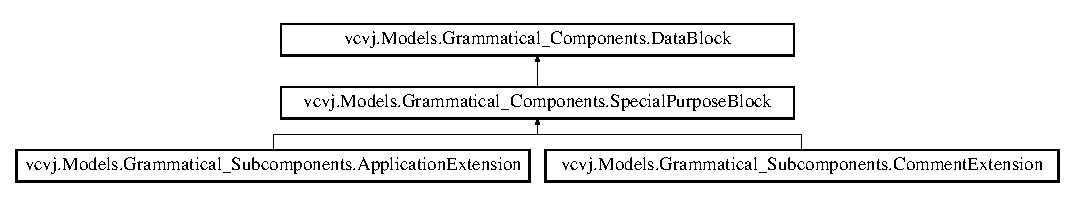
\includegraphics[height=2.216359cm]{classvcvj_1_1_models_1_1_grammatical___components_1_1_special_purpose_block}
\end{center}
\end{figure}
\subsection*{Public Member Functions}
\begin{DoxyCompactItemize}
\item 
\hyperlink{classvcvj_1_1_models_1_1_grammatical___subcomponents_1_1_application_extension}{Application\+Extension} {\bfseries To\+Application\+Extension} ()\hypertarget{classvcvj_1_1_models_1_1_grammatical___components_1_1_special_purpose_block_acf4bf6c98af6790d1b6362360aa4b9c0}{}\label{classvcvj_1_1_models_1_1_grammatical___components_1_1_special_purpose_block_acf4bf6c98af6790d1b6362360aa4b9c0}

\item 
\hyperlink{classvcvj_1_1_models_1_1_grammatical___subcomponents_1_1_comment_extension}{Comment\+Extension} {\bfseries To\+Comment\+Extension} ()\hypertarget{classvcvj_1_1_models_1_1_grammatical___components_1_1_special_purpose_block_a6a6edb15fa32b803f7b36eeceb06b648}{}\label{classvcvj_1_1_models_1_1_grammatical___components_1_1_special_purpose_block_a6a6edb15fa32b803f7b36eeceb06b648}

\end{DoxyCompactItemize}
\subsection*{Properties}
\begin{DoxyCompactItemize}
\item 
bool {\bfseries Is\+Application\+Extension}\hspace{0.3cm}{\ttfamily  \mbox{[}get\mbox{]}}\hypertarget{classvcvj_1_1_models_1_1_grammatical___components_1_1_special_purpose_block_a1067a5a9f73f041525fb145c80560b1e}{}\label{classvcvj_1_1_models_1_1_grammatical___components_1_1_special_purpose_block_a1067a5a9f73f041525fb145c80560b1e}

\item 
bool {\bfseries Is\+Comment\+Extension}\hspace{0.3cm}{\ttfamily  \mbox{[}get\mbox{]}}\hypertarget{classvcvj_1_1_models_1_1_grammatical___components_1_1_special_purpose_block_a534070d3a8fe216b7f2c7fbb037c1ed3}{}\label{classvcvj_1_1_models_1_1_grammatical___components_1_1_special_purpose_block_a534070d3a8fe216b7f2c7fbb037c1ed3}

\end{DoxyCompactItemize}


\subsection{Detailed Description}
Represents either an application extension or a comment extension. 



The documentation for this class was generated from the following file\+:\begin{DoxyCompactItemize}
\item 
vcvj/\+Models/\+Grammatical Components/Special\+Purpose\+Block.\+cs\end{DoxyCompactItemize}

\hypertarget{classvcvj_1_1_models_1_1_grammatical___components_1_1_table_based_image}{}\section{vcvj.\+Models.\+Grammatical\+\_\+\+Components.\+Table\+Based\+Image Class Reference}
\label{classvcvj_1_1_models_1_1_grammatical___components_1_1_table_based_image}\index{vcvj.\+Models.\+Grammatical\+\_\+\+Components.\+Table\+Based\+Image@{vcvj.\+Models.\+Grammatical\+\_\+\+Components.\+Table\+Based\+Image}}


A block containing an image descriptor, image data, and a local color table (optional).  


Inheritance diagram for vcvj.\+Models.\+Grammatical\+\_\+\+Components.\+Table\+Based\+Image\+:\begin{figure}[H]
\begin{center}
\leavevmode
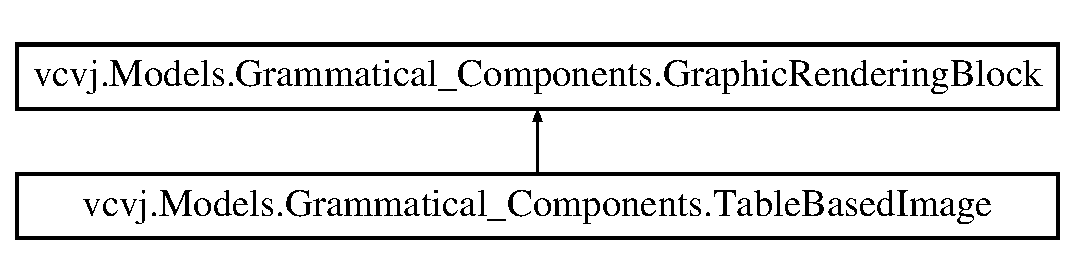
\includegraphics[height=2.000000cm]{classvcvj_1_1_models_1_1_grammatical___components_1_1_table_based_image}
\end{center}
\end{figure}
\subsection*{Properties}
\begin{DoxyCompactItemize}
\item 
\hyperlink{classvcvj_1_1_models_1_1_grammatical___subcomponents_1_1_image_descriptor}{Image\+Descriptor} {\bfseries Image\+Descriptor}\hspace{0.3cm}{\ttfamily  \mbox{[}get, set\mbox{]}}\hypertarget{classvcvj_1_1_models_1_1_grammatical___components_1_1_table_based_image_a9740ca8aa4e9541c58e1e57a3a044334}{}\label{classvcvj_1_1_models_1_1_grammatical___components_1_1_table_based_image_a9740ca8aa4e9541c58e1e57a3a044334}

\item 
\hyperlink{classvcvj_1_1_models_1_1_grammatical___subcomponents_1_1_local_color_table}{Local\+Color\+Table} {\bfseries Local\+Color\+Table}\hspace{0.3cm}{\ttfamily  \mbox{[}get, set\mbox{]}}\hypertarget{classvcvj_1_1_models_1_1_grammatical___components_1_1_table_based_image_a859e4ff577588d8e15242fb4e7b12769}{}\label{classvcvj_1_1_models_1_1_grammatical___components_1_1_table_based_image_a859e4ff577588d8e15242fb4e7b12769}

\item 
\hyperlink{classvcvj_1_1_models_1_1_grammatical___subcomponents_1_1_image_data}{Image\+Data} {\bfseries Image\+Data}\hspace{0.3cm}{\ttfamily  \mbox{[}get, set\mbox{]}}\hypertarget{classvcvj_1_1_models_1_1_grammatical___components_1_1_table_based_image_ab96897d307dfe65b8c53cbf4bfb4cb64}{}\label{classvcvj_1_1_models_1_1_grammatical___components_1_1_table_based_image_ab96897d307dfe65b8c53cbf4bfb4cb64}

\end{DoxyCompactItemize}
\subsection*{Additional Inherited Members}


\subsection{Detailed Description}
A block containing an image descriptor, image data, and a local color table (optional). 



The documentation for this class was generated from the following file\+:\begin{DoxyCompactItemize}
\item 
vcvj/\+Models/\+Grammatical Components/Table\+Based\+Image.\+cs\end{DoxyCompactItemize}

\hypertarget{classvcvj_1_1_models_1_1_grammatical___subcomponents_1_1_trailer}{}\section{vcvj.\+Models.\+Grammatical\+\_\+\+Subcomponents.\+Trailer Class Reference}
\label{classvcvj_1_1_models_1_1_grammatical___subcomponents_1_1_trailer}\index{vcvj.\+Models.\+Grammatical\+\_\+\+Subcomponents.\+Trailer@{vcvj.\+Models.\+Grammatical\+\_\+\+Subcomponents.\+Trailer}}


The image\textquotesingle{}s trailer marker.  


\subsection*{Public Member Functions}
\begin{DoxyCompactItemize}
\item 
\hyperlink{classvcvj_1_1_models_1_1_grammatical___subcomponents_1_1_trailer_ab118002aebcca587e251ae6864f290a7}{Trailer} (byte b)
\begin{DoxyCompactList}\small\item\em Populates the image\textquotesingle{}s trailer, denoting the end of the data stream. \end{DoxyCompactList}\end{DoxyCompactItemize}
\subsection*{Public Attributes}
\begin{DoxyCompactItemize}
\item 
const int {\bfseries Total\+Block\+Length} = 1\hypertarget{classvcvj_1_1_models_1_1_grammatical___subcomponents_1_1_trailer_a15ebcc9e920e57c56924ffc0cf3815d2}{}\label{classvcvj_1_1_models_1_1_grammatical___subcomponents_1_1_trailer_a15ebcc9e920e57c56924ffc0cf3815d2}

\item 
byte\mbox{[}$\,$\mbox{]} {\bfseries Bytes} = new byte\mbox{[}Trailer.\+Total\+Block\+Length\mbox{]}\hypertarget{classvcvj_1_1_models_1_1_grammatical___subcomponents_1_1_trailer_a6b063b6a4b09044b06de6089f8defb61}{}\label{classvcvj_1_1_models_1_1_grammatical___subcomponents_1_1_trailer_a6b063b6a4b09044b06de6089f8defb61}

\end{DoxyCompactItemize}
\subsection*{Properties}
\begin{DoxyCompactItemize}
\item 
byte {\bfseries Marker}\hspace{0.3cm}{\ttfamily  \mbox{[}get, set\mbox{]}}\hypertarget{classvcvj_1_1_models_1_1_grammatical___subcomponents_1_1_trailer_a6cc95c6b7466d1fd5b2da944b95d3586}{}\label{classvcvj_1_1_models_1_1_grammatical___subcomponents_1_1_trailer_a6cc95c6b7466d1fd5b2da944b95d3586}

\end{DoxyCompactItemize}


\subsection{Detailed Description}
The image\textquotesingle{}s trailer marker. 



\subsection{Constructor \& Destructor Documentation}
\index{vcvj\+::\+Models\+::\+Grammatical\+\_\+\+Subcomponents\+::\+Trailer@{vcvj\+::\+Models\+::\+Grammatical\+\_\+\+Subcomponents\+::\+Trailer}!Trailer@{Trailer}}
\index{Trailer@{Trailer}!vcvj\+::\+Models\+::\+Grammatical\+\_\+\+Subcomponents\+::\+Trailer@{vcvj\+::\+Models\+::\+Grammatical\+\_\+\+Subcomponents\+::\+Trailer}}
\subsubsection[{\texorpdfstring{Trailer(byte b)}{Trailer(byte b)}}]{\setlength{\rightskip}{0pt plus 5cm}vcvj.\+Models.\+Grammatical\+\_\+\+Subcomponents.\+Trailer.\+Trailer (
\begin{DoxyParamCaption}
\item[{byte}]{b}
\end{DoxyParamCaption}
)\hspace{0.3cm}{\ttfamily [inline]}}\hypertarget{classvcvj_1_1_models_1_1_grammatical___subcomponents_1_1_trailer_ab118002aebcca587e251ae6864f290a7}{}\label{classvcvj_1_1_models_1_1_grammatical___subcomponents_1_1_trailer_ab118002aebcca587e251ae6864f290a7}


Populates the image\textquotesingle{}s trailer, denoting the end of the data stream. 



The documentation for this class was generated from the following file\+:\begin{DoxyCompactItemize}
\item 
vcvj/\+Models/\+Grammatical Subcomponents/Trailer.\+cs\end{DoxyCompactItemize}

\hypertarget{classvcvj_1_1_exceptions_1_1_unidentified_block_exception}{}\section{vcvj.\+Exceptions.\+Unidentified\+Block\+Exception Class Reference}
\label{classvcvj_1_1_exceptions_1_1_unidentified_block_exception}\index{vcvj.\+Exceptions.\+Unidentified\+Block\+Exception@{vcvj.\+Exceptions.\+Unidentified\+Block\+Exception}}
Inheritance diagram for vcvj.\+Exceptions.\+Unidentified\+Block\+Exception\+:\begin{figure}[H]
\begin{center}
\leavevmode
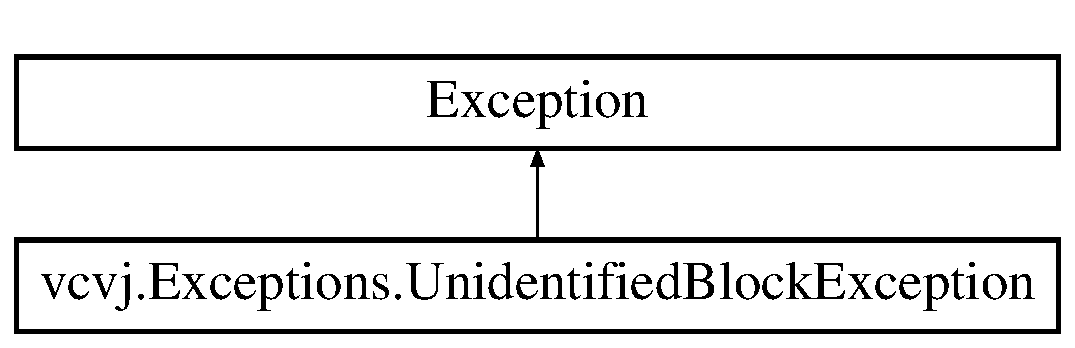
\includegraphics[height=2.000000cm]{classvcvj_1_1_exceptions_1_1_unidentified_block_exception}
\end{center}
\end{figure}
\subsection*{Public Member Functions}
\begin{DoxyCompactItemize}
\item 
{\bfseries Unidentified\+Block\+Exception} (string message)\hypertarget{classvcvj_1_1_exceptions_1_1_unidentified_block_exception_a8c33f3e8a5d61834e04229dd77a552c3}{}\label{classvcvj_1_1_exceptions_1_1_unidentified_block_exception_a8c33f3e8a5d61834e04229dd77a552c3}

\item 
{\bfseries Unidentified\+Block\+Exception} (string message, Exception inner)\hypertarget{classvcvj_1_1_exceptions_1_1_unidentified_block_exception_aff570dbd1eb13e62f9db98f1eaf4c041}{}\label{classvcvj_1_1_exceptions_1_1_unidentified_block_exception_aff570dbd1eb13e62f9db98f1eaf4c041}

\end{DoxyCompactItemize}


The documentation for this class was generated from the following file\+:\begin{DoxyCompactItemize}
\item 
vcvj/\+Exceptions/Unidentified\+Block\+Exception.\+cs\end{DoxyCompactItemize}

\hypertarget{classvcvj_1_1_vcvj_image}{}\section{vcvj.\+Vcvj\+Image Class Reference}
\label{classvcvj_1_1_vcvj_image}\index{vcvj.\+Vcvj\+Image@{vcvj.\+Vcvj\+Image}}
\subsection*{Public Member Functions}
\begin{DoxyCompactItemize}
\item 
void \hyperlink{classvcvj_1_1_vcvj_image_a8dfb7a8003fb52fe79c68fab3bfa4dec}{Compile\+Byte\+Array} ()
\begin{DoxyCompactList}\small\item\em Compiles the parsed tokens/components back into a byte array. \end{DoxyCompactList}\item 
void \hyperlink{classvcvj_1_1_vcvj_image_a9f88afceee83616e2e151ebc2029517a}{Save} (string suffix=\char`\"{}\char`\"{}, bool overwrite\+Existing\+Image=false)
\begin{DoxyCompactList}\small\item\em Saves the image to the source image folder, using the name of the original source image and an optional suffix to append to the output file. \end{DoxyCompactList}\item 
void \hyperlink{classvcvj_1_1_vcvj_image_a692bb3dc3559a89e866eacc78cb11c6d}{Save\+To\+Path} (string filepath, bool overwrite\+Existing\+Image=false)
\begin{DoxyCompactList}\small\item\em Saves the image to a fully qualified path. \end{DoxyCompactList}\item 
void \hyperlink{classvcvj_1_1_vcvj_image_a3672c362bd1e1422d7f2eae41e58bb2a}{Compile\+And\+Save} (string suffix=\char`\"{}\char`\"{}, bool overwrite\+Existing\+Image=false)
\begin{DoxyCompactList}\small\item\em Compiles the data stream and saves the image to the input folder with a new file name. \end{DoxyCompactList}\item 
void \hyperlink{classvcvj_1_1_vcvj_image_a92d372f81cb9dceb2d644f6f13c1d5bc}{Compile\+And\+Save\+To\+Path} (string file\+Path, bool overwrite\+Existing\+Image=false)
\begin{DoxyCompactList}\small\item\em Compiles the data stream and saves the image to a fully qualified path. \end{DoxyCompactList}\item 
\hyperlink{classvcvj_1_1_vcvj_image_a5d9a5ea2928dd78e3c1899dc6a83732a}{Vcvj\+Image} (string input\+File\+Path)
\begin{DoxyCompactList}\small\item\em Creates a new Vc\+Vj\+Image object from a G\+IF image located at the specified file path. \end{DoxyCompactList}\item 
\hyperlink{classvcvj_1_1_vcvj_image_afdfa6f404bed3a3c0a0c9a16060206f8}{Vcvj\+Image} (string folder\+Name, string file\+Name)
\begin{DoxyCompactList}\small\item\em Creates a new Vc\+Vj\+Image object from a G\+IF image located at the specified folder with the specified file name. \end{DoxyCompactList}\end{DoxyCompactItemize}
\subsection*{Properties}
\begin{DoxyCompactItemize}
\item 
string \hyperlink{classvcvj_1_1_vcvj_image_a2a21889ea8a2dac7832e69b224e47732}{Input\+Folder\+Name}\hspace{0.3cm}{\ttfamily  \mbox{[}get, set\mbox{]}}
\begin{DoxyCompactList}\small\item\em The name of the folder that the source image is located in. \end{DoxyCompactList}\item 
string \hyperlink{classvcvj_1_1_vcvj_image_a34afafb554b739cd21a3ad8b71007462}{Input\+File\+Name}\hspace{0.3cm}{\ttfamily  \mbox{[}get, set\mbox{]}}
\begin{DoxyCompactList}\small\item\em The name of the source image file (excluding extension). \end{DoxyCompactList}\item 
string {\bfseries Input\+File\+Path}\hspace{0.3cm}{\ttfamily  \mbox{[}get\mbox{]}}\hypertarget{classvcvj_1_1_vcvj_image_adba0cc00bee473c2737a0a8de9ef10ec}{}\label{classvcvj_1_1_vcvj_image_adba0cc00bee473c2737a0a8de9ef10ec}

\item 
\hyperlink{classvcvj_1_1_models_1_1_grammatical___components_1_1_data_stream}{Data\+Stream} \hyperlink{classvcvj_1_1_vcvj_image_af7be319d59a08f70d624631d8f1bccbd}{Data\+Stream}\hspace{0.3cm}{\ttfamily  \mbox{[}get, set\mbox{]}}
\begin{DoxyCompactList}\small\item\em Represents the tokenized G\+IF image\textquotesingle{}s constituent tokens. \end{DoxyCompactList}\end{DoxyCompactItemize}


\subsection{Constructor \& Destructor Documentation}
\index{vcvj\+::\+Vcvj\+Image@{vcvj\+::\+Vcvj\+Image}!Vcvj\+Image@{Vcvj\+Image}}
\index{Vcvj\+Image@{Vcvj\+Image}!vcvj\+::\+Vcvj\+Image@{vcvj\+::\+Vcvj\+Image}}
\subsubsection[{\texorpdfstring{Vcvj\+Image(string input\+File\+Path)}{VcvjImage(string inputFilePath)}}]{\setlength{\rightskip}{0pt plus 5cm}vcvj.\+Vcvj\+Image.\+Vcvj\+Image (
\begin{DoxyParamCaption}
\item[{string}]{input\+File\+Path}
\end{DoxyParamCaption}
)\hspace{0.3cm}{\ttfamily [inline]}}\hypertarget{classvcvj_1_1_vcvj_image_a5d9a5ea2928dd78e3c1899dc6a83732a}{}\label{classvcvj_1_1_vcvj_image_a5d9a5ea2928dd78e3c1899dc6a83732a}


Creates a new Vc\+Vj\+Image object from a G\+IF image located at the specified file path. 


\begin{DoxyParams}{Parameters}
{\em filename} & The fully qualified path to the file.\\
\hline
\end{DoxyParams}
\index{vcvj\+::\+Vcvj\+Image@{vcvj\+::\+Vcvj\+Image}!Vcvj\+Image@{Vcvj\+Image}}
\index{Vcvj\+Image@{Vcvj\+Image}!vcvj\+::\+Vcvj\+Image@{vcvj\+::\+Vcvj\+Image}}
\subsubsection[{\texorpdfstring{Vcvj\+Image(string folder\+Name, string file\+Name)}{VcvjImage(string folderName, string fileName)}}]{\setlength{\rightskip}{0pt plus 5cm}vcvj.\+Vcvj\+Image.\+Vcvj\+Image (
\begin{DoxyParamCaption}
\item[{string}]{folder\+Name, }
\item[{string}]{file\+Name}
\end{DoxyParamCaption}
)\hspace{0.3cm}{\ttfamily [inline]}}\hypertarget{classvcvj_1_1_vcvj_image_afdfa6f404bed3a3c0a0c9a16060206f8}{}\label{classvcvj_1_1_vcvj_image_afdfa6f404bed3a3c0a0c9a16060206f8}


Creates a new Vc\+Vj\+Image object from a G\+IF image located at the specified folder with the specified file name. 


\begin{DoxyParams}{Parameters}
{\em folder\+Name} & The folder containing the G\+IF file (including trailing backslash, e.\+g. \textquotesingle{}C\+:\textbackslash{}\textquotesingle{}).\\
\hline
{\em file\+Name} & The name of the G\+IF file (including the extension, e.\+g. \textquotesingle{}Balloons.\+gif\textquotesingle{}).\\
\hline
\end{DoxyParams}


\subsection{Member Function Documentation}
\index{vcvj\+::\+Vcvj\+Image@{vcvj\+::\+Vcvj\+Image}!Compile\+And\+Save@{Compile\+And\+Save}}
\index{Compile\+And\+Save@{Compile\+And\+Save}!vcvj\+::\+Vcvj\+Image@{vcvj\+::\+Vcvj\+Image}}
\subsubsection[{\texorpdfstring{Compile\+And\+Save(string suffix="""", bool overwrite\+Existing\+Image=false)}{CompileAndSave(string suffix="", bool overwriteExistingImage=false)}}]{\setlength{\rightskip}{0pt plus 5cm}void vcvj.\+Vcvj\+Image.\+Compile\+And\+Save (
\begin{DoxyParamCaption}
\item[{string}]{suffix = {\ttfamily \char`\"{}\char`\"{}}, }
\item[{bool}]{overwrite\+Existing\+Image = {\ttfamily false}}
\end{DoxyParamCaption}
)\hspace{0.3cm}{\ttfamily [inline]}}\hypertarget{classvcvj_1_1_vcvj_image_a3672c362bd1e1422d7f2eae41e58bb2a}{}\label{classvcvj_1_1_vcvj_image_a3672c362bd1e1422d7f2eae41e58bb2a}


Compiles the data stream and saves the image to the input folder with a new file name. 


\begin{DoxyParams}{Parameters}
{\em overwrite\+Existing\+Image} & Overwrites the existing image located at the new file path (default == false).\\
\hline
{\em suffix} & An optional suffix to append to the end of the new file name (e.\+g. \textquotesingle{} -\/ modified\textquotesingle{}).\\
\hline
\end{DoxyParams}
\index{vcvj\+::\+Vcvj\+Image@{vcvj\+::\+Vcvj\+Image}!Compile\+And\+Save\+To\+Path@{Compile\+And\+Save\+To\+Path}}
\index{Compile\+And\+Save\+To\+Path@{Compile\+And\+Save\+To\+Path}!vcvj\+::\+Vcvj\+Image@{vcvj\+::\+Vcvj\+Image}}
\subsubsection[{\texorpdfstring{Compile\+And\+Save\+To\+Path(string file\+Path, bool overwrite\+Existing\+Image=false)}{CompileAndSaveToPath(string filePath, bool overwriteExistingImage=false)}}]{\setlength{\rightskip}{0pt plus 5cm}void vcvj.\+Vcvj\+Image.\+Compile\+And\+Save\+To\+Path (
\begin{DoxyParamCaption}
\item[{string}]{file\+Path, }
\item[{bool}]{overwrite\+Existing\+Image = {\ttfamily false}}
\end{DoxyParamCaption}
)\hspace{0.3cm}{\ttfamily [inline]}}\hypertarget{classvcvj_1_1_vcvj_image_a92d372f81cb9dceb2d644f6f13c1d5bc}{}\label{classvcvj_1_1_vcvj_image_a92d372f81cb9dceb2d644f6f13c1d5bc}


Compiles the data stream and saves the image to a fully qualified path. 


\begin{DoxyParams}{Parameters}
{\em overwrite\+Existing\+Image} & Overwrites the existing image located at the new file path (default == false).\\
\hline
{\em file\+Path} & The fully qualified path to the new file (e.\+g. \textquotesingle{}C\+:.gif\textquotesingle{}).\\
\hline
\end{DoxyParams}
\index{vcvj\+::\+Vcvj\+Image@{vcvj\+::\+Vcvj\+Image}!Compile\+Byte\+Array@{Compile\+Byte\+Array}}
\index{Compile\+Byte\+Array@{Compile\+Byte\+Array}!vcvj\+::\+Vcvj\+Image@{vcvj\+::\+Vcvj\+Image}}
\subsubsection[{\texorpdfstring{Compile\+Byte\+Array()}{CompileByteArray()}}]{\setlength{\rightskip}{0pt plus 5cm}void vcvj.\+Vcvj\+Image.\+Compile\+Byte\+Array (
\begin{DoxyParamCaption}
{}
\end{DoxyParamCaption}
)\hspace{0.3cm}{\ttfamily [inline]}}\hypertarget{classvcvj_1_1_vcvj_image_a8dfb7a8003fb52fe79c68fab3bfa4dec}{}\label{classvcvj_1_1_vcvj_image_a8dfb7a8003fb52fe79c68fab3bfa4dec}


Compiles the parsed tokens/components back into a byte array. 

\index{vcvj\+::\+Vcvj\+Image@{vcvj\+::\+Vcvj\+Image}!Save@{Save}}
\index{Save@{Save}!vcvj\+::\+Vcvj\+Image@{vcvj\+::\+Vcvj\+Image}}
\subsubsection[{\texorpdfstring{Save(string suffix="""", bool overwrite\+Existing\+Image=false)}{Save(string suffix="", bool overwriteExistingImage=false)}}]{\setlength{\rightskip}{0pt plus 5cm}void vcvj.\+Vcvj\+Image.\+Save (
\begin{DoxyParamCaption}
\item[{string}]{suffix = {\ttfamily \char`\"{}\char`\"{}}, }
\item[{bool}]{overwrite\+Existing\+Image = {\ttfamily false}}
\end{DoxyParamCaption}
)\hspace{0.3cm}{\ttfamily [inline]}}\hypertarget{classvcvj_1_1_vcvj_image_a9f88afceee83616e2e151ebc2029517a}{}\label{classvcvj_1_1_vcvj_image_a9f88afceee83616e2e151ebc2029517a}


Saves the image to the source image folder, using the name of the original source image and an optional suffix to append to the output file. 


\begin{DoxyParams}{Parameters}
{\em suffix} & An optional suffix to append to the end of the new file name (e.\+g. \textquotesingle{} -\/ modified\textquotesingle{}).\\
\hline
{\em overwrite\+Existing\+Image} & Overwrites the existing image located at the new file path (default == false).\\
\hline
\end{DoxyParams}
\index{vcvj\+::\+Vcvj\+Image@{vcvj\+::\+Vcvj\+Image}!Save\+To\+Path@{Save\+To\+Path}}
\index{Save\+To\+Path@{Save\+To\+Path}!vcvj\+::\+Vcvj\+Image@{vcvj\+::\+Vcvj\+Image}}
\subsubsection[{\texorpdfstring{Save\+To\+Path(string filepath, bool overwrite\+Existing\+Image=false)}{SaveToPath(string filepath, bool overwriteExistingImage=false)}}]{\setlength{\rightskip}{0pt plus 5cm}void vcvj.\+Vcvj\+Image.\+Save\+To\+Path (
\begin{DoxyParamCaption}
\item[{string}]{filepath, }
\item[{bool}]{overwrite\+Existing\+Image = {\ttfamily false}}
\end{DoxyParamCaption}
)\hspace{0.3cm}{\ttfamily [inline]}}\hypertarget{classvcvj_1_1_vcvj_image_a692bb3dc3559a89e866eacc78cb11c6d}{}\label{classvcvj_1_1_vcvj_image_a692bb3dc3559a89e866eacc78cb11c6d}


Saves the image to a fully qualified path. 


\begin{DoxyParams}{Parameters}
{\em filepath} & The fully qualified path to the new file (e.\+g. \textquotesingle{}C\+:.gif\textquotesingle{}).\\
\hline
{\em overwrite\+Existing\+Image} & Overwrites the existing image located at the new file path (default == false).\\
\hline
\end{DoxyParams}


\subsection{Property Documentation}
\index{vcvj\+::\+Vcvj\+Image@{vcvj\+::\+Vcvj\+Image}!Data\+Stream@{Data\+Stream}}
\index{Data\+Stream@{Data\+Stream}!vcvj\+::\+Vcvj\+Image@{vcvj\+::\+Vcvj\+Image}}
\subsubsection[{\texorpdfstring{Data\+Stream}{DataStream}}]{\setlength{\rightskip}{0pt plus 5cm}{\bf Data\+Stream} vcvj.\+Vcvj\+Image.\+Data\+Stream\hspace{0.3cm}{\ttfamily [get]}, {\ttfamily [set]}}\hypertarget{classvcvj_1_1_vcvj_image_af7be319d59a08f70d624631d8f1bccbd}{}\label{classvcvj_1_1_vcvj_image_af7be319d59a08f70d624631d8f1bccbd}


Represents the tokenized G\+IF image\textquotesingle{}s constituent tokens. 

\index{vcvj\+::\+Vcvj\+Image@{vcvj\+::\+Vcvj\+Image}!Input\+File\+Name@{Input\+File\+Name}}
\index{Input\+File\+Name@{Input\+File\+Name}!vcvj\+::\+Vcvj\+Image@{vcvj\+::\+Vcvj\+Image}}
\subsubsection[{\texorpdfstring{Input\+File\+Name}{InputFileName}}]{\setlength{\rightskip}{0pt plus 5cm}string vcvj.\+Vcvj\+Image.\+Input\+File\+Name\hspace{0.3cm}{\ttfamily [get]}, {\ttfamily [set]}}\hypertarget{classvcvj_1_1_vcvj_image_a34afafb554b739cd21a3ad8b71007462}{}\label{classvcvj_1_1_vcvj_image_a34afafb554b739cd21a3ad8b71007462}


The name of the source image file (excluding extension). 

\index{vcvj\+::\+Vcvj\+Image@{vcvj\+::\+Vcvj\+Image}!Input\+Folder\+Name@{Input\+Folder\+Name}}
\index{Input\+Folder\+Name@{Input\+Folder\+Name}!vcvj\+::\+Vcvj\+Image@{vcvj\+::\+Vcvj\+Image}}
\subsubsection[{\texorpdfstring{Input\+Folder\+Name}{InputFolderName}}]{\setlength{\rightskip}{0pt plus 5cm}string vcvj.\+Vcvj\+Image.\+Input\+Folder\+Name\hspace{0.3cm}{\ttfamily [get]}, {\ttfamily [set]}}\hypertarget{classvcvj_1_1_vcvj_image_a2a21889ea8a2dac7832e69b224e47732}{}\label{classvcvj_1_1_vcvj_image_a2a21889ea8a2dac7832e69b224e47732}


The name of the folder that the source image is located in. 



The documentation for this class was generated from the following file\+:\begin{DoxyCompactItemize}
\item 
vcvj/Vcvj\+Image.\+cs\end{DoxyCompactItemize}

%--- End generated contents ---

% Index
\backmatter
\newpage
\phantomsection
\clearemptydoublepage
\addcontentsline{toc}{chapter}{Index}
\printindex

\end{document}
